%% The following is a directive for TeXShop to indicate the main file
%%!TEX root = diss.tex

\chapter{A Mapping of 3D Reconstruction}
\label{ch:3DRecon_Mapping}
Most of the vision work focuses on developing algorithmic novelties, and very few investigates the rigorous conditions under which these algorithms work. Thus this knowledge is only known empirically, without a rigorous definition of the application domain or problem conditions. This section builds upon the 3D description proposed in Chapter~\ref{ch:3DRecon_Desc}, and attempts to find out the optimal algorithms under a well defined condition.

To achieve this goal, we need a dataset to evaluate the performance of each algorithm under varied conditions, which is not the goal of most online datasets. To the best of our knowledge, current existing 3D benchmarks focus on one specific class of algorithms, for example, the Middlebury dataset is targeted at MVS algorithms, and the `DiLiGenT' dataset is for Photometric Stereo algorithms. This makes them only suitable to the evaluation of the within-category algorithms. There is no dataset that evaluates 3D reconstruction across differ categories, not to mention one that covers a range of properties of material and geometry and all their combinations. The reasons for the lack of such a dataset are: 1). it's already tedious to create a real-world dataset for one specific category of algorithms, it would be even more challenging to create a dataset for a larger range of algorithms with the ground truth; 2). it's practically impossible to change one property, \eg, noise level, lighting configuration, material, \etc while fixing the others in order to conduct a thorough evaluation.

We propose a synthetic dataset created by phisically-based rendering software - Blender, to evaluate the 3D reconstruction algorithms. The dataset includes a collection of images of a scene under different materials or lighting conditions. The camera/projector intrinsic and extrinsic parameters are computed directly from the configurations of the synthetic setup, and the ground truth, including the 3D model point cloud and normal map, are generated directly from Blender.

\section{Synthetic setup}
We use the physically-based rendering engine named Cycles in Blender to generate the synthetic dataset. For each technique, the configuration of the camera remains fixed. The image resolution is 1280$\times$720, with a focal length of $35mm$ or $1400pix$.

For the Multi-View Stereo setup, there are five rings of cameras, of which the elevation angle is $15^\circ$, $30^\circ$, $45^\circ$, $60^\circ$, $90^\circ$. The between-angle of two neighbouring cameras is $30^\circ$, $30^\circ$, $45^\circ$, $45^\circ$, and $360^\circ$. Thus there are in total $12+12+8+8+1=41$ cameras.

For the photometric stereo setup, since increasing the number of images is only important up to a point, the experimental results showed that most algorithms reaches to optimum when 15 images are used~\cite{Berkiten:2016:ARB}. To make a balance between algorithm performance and rendering time, we use 25 light sources, which are distributed on four different rings with elevation angle of $90^\circ$, $85^\circ$, $60^\circ$, and $45^\circ$. The azimuth angle between two neighbouring light sources is $45^\circ$.

For the structured light setup, the baseline angle between the camera and the projector is $10^\circ$, and only one camera is used, thus only a portion of the object is visible. The resolution of the projector is $1024\times768$, thus 10 Gray code patterns are needed. To counter the effect of inter-reflection, each pattern and its inverse are projected, which makes it less sensitive to scattered light.

\section{Structure of Datasets}
Due to the number of properties and number of levels for each property, it would be unrealistic to render all their combinations. For instance, if there are $N$ properties and each is discretized into $L$ levels, the number of different combinations is $L^N$, and for each combination, there are in total $41+25+42=108$ images to render. Therefore, we take another approach: 1). we investigate the \textit{effetive problem domain} which consists of only the \textit{effective} and \textit{dependent} properties; 2). generate synthetic images for the \textit{effective} and \textit{dependent} properties and all their combinations. The structure of the dataset is as follows
\begin{figure}[!htbp]
\centering
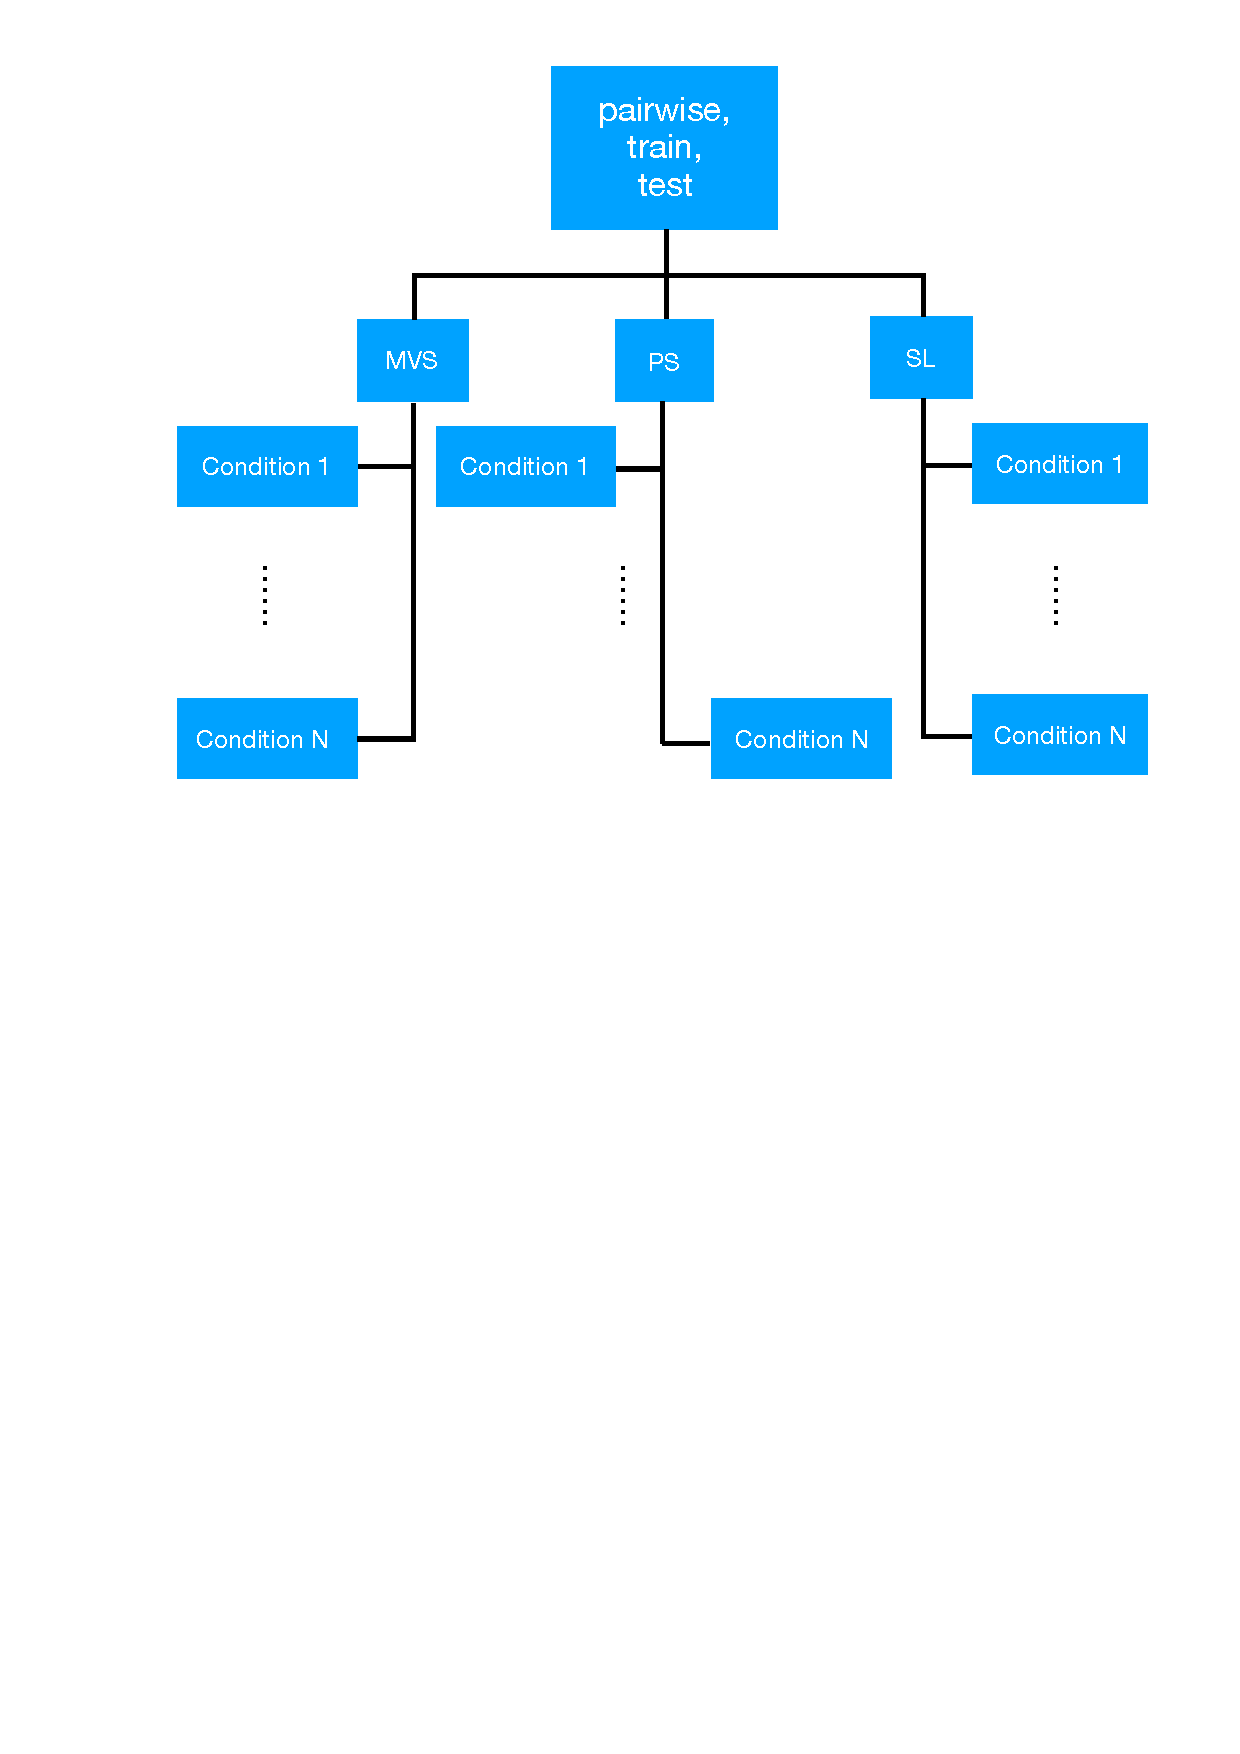
\includegraphics[width=0.5\textwidth]{mapping/dataset_structure}
\caption{Structure of the synthetic dataset.}
\label{fig:dataset_structure}
\end{figure}

\section{Evaluation metrics}
We use the metric proposed in \cite{seitz2006comparison} to evaluate MVS and SL algorithms. More specifically, we compute the accuracy and completeness of the reconstruction. For accuracy, the distance between the points in the reconstruction $R$ and the nearest points on ground truth $G$ is computed, and the distance $d$ such that $X\%$ of the points on $R$ are within distance $d$ of $G$ is considered as accuracy. Thus the lower the accuracy value, the better the reconstruction result. For completeness, we compute the distance from $G$ to $R$. Intuitively, points on $G$ is not ``covered'' if no suitable nearest points on $R$ found. A more practical approach computes the fraction of points of $G$ that are within an allowable distance $d$ of $R$.
Note that as the reconstruction gets better, the ``accuracy value'' goes down, but the ``accuracy'' is often claimed as improved, which is contradictory at first glance. To make it more consistent to the natural context, we say the accuracy goes up when the reconstruction gets better.

For photometric stereo, the depth information is lost since only one viewpoint is used. Thus the previous metrics are not applicable. We employ another evaluation criteria that is widely adopted by the community, which is based on the statistics of angular error. For each pixel, the angular error is calculated as the angle between the estimated and ground truth normal, \ie $arccos$($n_g^T n$), where $n_g$ and $n$ is the ground truth and estimated normals respectively. In addition to the mean angular error, we also calculate the standard deviation, minimum, maximum, median, the first quartile, and the third quartile of angular errors for each estimated normal map.

\section{Selected methods}
We have selected one representative algorithm from three major classes of algorithms presented in Chapter~\ref{ch:3DRecon_Taxo}: the PMVS proposed in~\cite{furukawa2010accurate}, the example-based photometric stereo proposed in~\cite{hertzmann2005example}, and the Gray code structured light technique, see Table~\ref{tab:selected_algos} for a summary of the selected algorithms. The current implementation of SL projects both column and row patterns, and depth values are computed using these two kinds of patterns individually. A depth consistency checking step is performed to reject erroneous triangulations.
\begin{table}[!htbp]
\centering
\begin{tabular}{c|c|c|c|c}
\hline
Technique & Texture & Albedeo & Specular & Roughness\\
\hline\hline
\multicolumn{5}{l}{PMVS: patch-based, seed points propagation MVS.}\\
\hline
PMVS & High & - & Low & -\\
\hline\hline
\multicolumn{5}{l}{EPS: example-based Photometric Stereo}\\
\hline
EPS & - & High & Low & High \\
\hline\hline
\multicolumn{5}{l}{GSL: Gray code Structured Light technique}\\
\hline
GSL & - & High & Low & High\\
\hline
\end{tabular}
\caption{Summary of the selected algorithms for the framework, and the corresponding working conditions in theory.}
\label{tab:selected_algos}
\end{table}

\section{Baseline}
\begin{table}[!htbp]
\centering
\begin{tabular}{c|c|c|c|c}
\hline
Technique & Texture & Albedeo & Specular & Roughness\\
\hline\hline
\multicolumn{5}{l}{VH: volumetric Visual Hull}\\
\hline
VH & - & - & - & -\\
\hline\hline
\multicolumn{5}{l}{LLS-PS: linear least squares Photometric Stereo.}\\
\hline
LLS-PS & - & High & Low & High\\
\hline
\end{tabular}
\caption{Summary of the baseline algorithms for the framework, and the corresponding working conditions in theory.}
\label{tab:selected_baseline_algos}
\end{table}
A baseline algorithm that works sufficiently well under most conditions should be chosen so that it's possible to determine the performance of selected algorithm within the framework. We choose the Visual Hull technique as one of our baseline algorithms since 1) it works relatively well as long as the silhouette of the object can be reliably extracted thus is insensitive to material properties; 2). the true scene is always enclosed by the reconstruction result thus the outcome is always predictable.

A simple linear least squares based Photometric Stereo (LLS-PS) is selected to evaluate Photometric Stereo algorithms. However, there is currently no such algorithm that works reasonaly well under various conditions. Thus we run this baseline algorithm under the optimal condition to ensure that a best possible result is achieved. To assess the performance of the selected PS algorithm against the baseline, we compare the following characteristics of the angular error:

\subsubsection{Measures of Central Tendency}
Mean and median are both valid measures of central tendency. But as the skewness increases, mean would be dragged in the direct of the skew, thus the median is generally considered to be the best representative of the central location of the data. The more skewed the distribution, the greater the difference between the median and mean, and the greater emphasis should be placed on using the median as opposed to the mean. See Figure~\ref{fig:ang_diff_skew}.
\begin{figure}[!htbp]
\centering
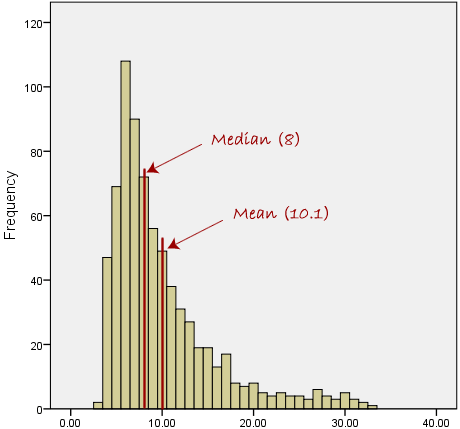
\includegraphics[width=0.4\textwidth]{mapping/skewed}
\caption{A right-skewed distribution, which is a typical graph of the angular error.}
\label{fig:ang_diff_skew}
\end{figure}

\subsubsection{Variation}
\begin{itemize}
  \item Interquatile range %: $Q_{(3 - 1)} < 3$;
  \item Standard deviation %: canslightly larger than $Q_3$
\end{itemize}
  
\subsubsection{Skewness (right/positive-skewness)}
The normal estimation is more insensitive to angular error when the mean and median are close. The shape can be relatively well recovered with a mean/median angular error of $10^\circ$, see Figure~\ref{fig:ps_criteria} (a)-(f). The normal estimation becomes more susceptible as the difference between the mean and median increases, see Figure~\ref{fig:ps_criteria} (g)-(l). This can be explained as follows: when the normals are reliably estimated, the angular error should follow a Gaussian distribution. Therefore, the mean and median are close to each other. However, if normals are poorly recovering, the mean would become larger since large angular errors exist while the median would change far less since only a small amount of pixels are affected. Thus the difference beteen mean and median would be larger when surface normals are poorly recovered.

\begin{figure}[!htbp]
\begin{tabular}{ccc}
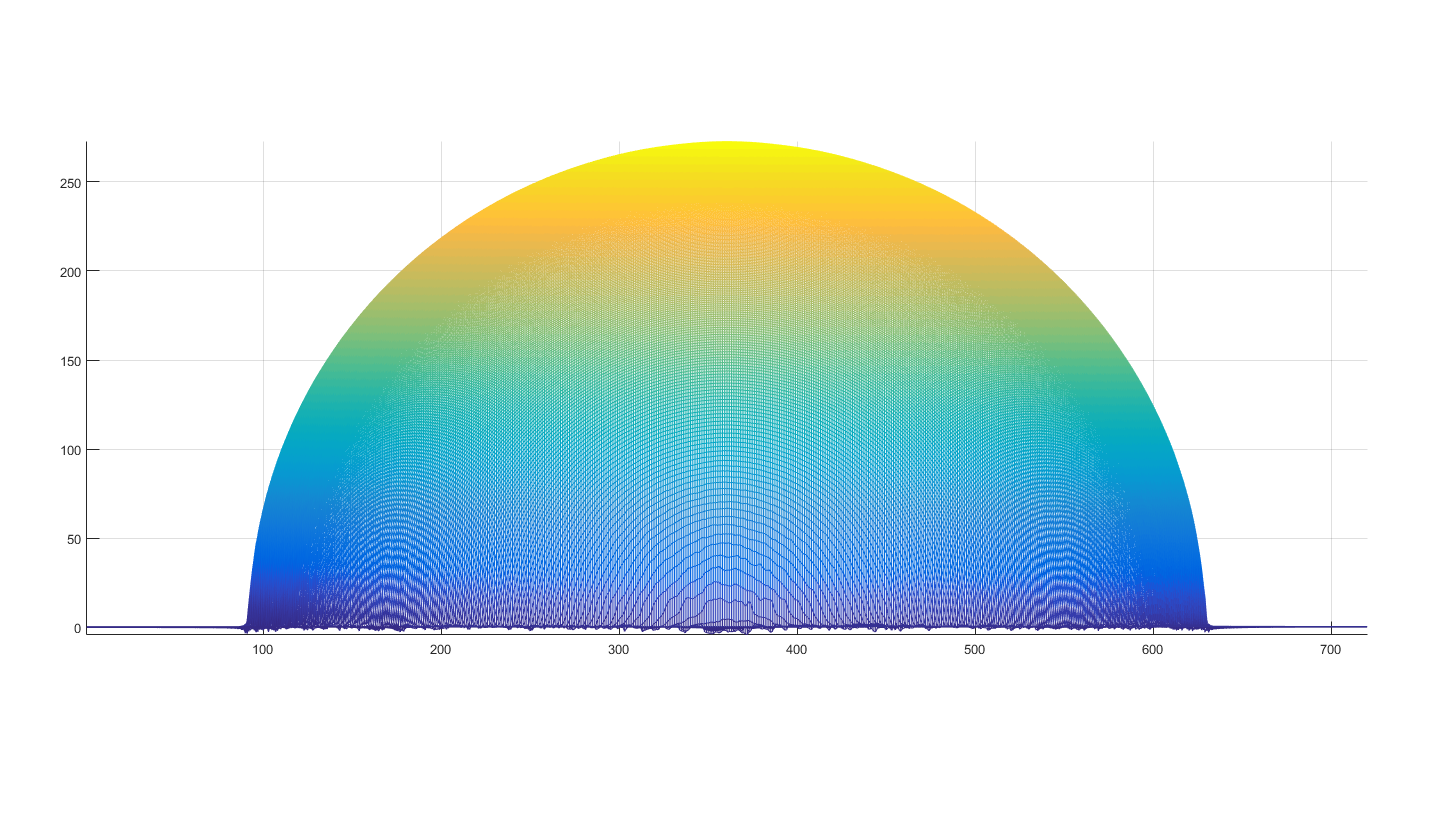
\includegraphics[width=0.33\textwidth]{mapping/ps_criteria/mu_med_0_0.png} &
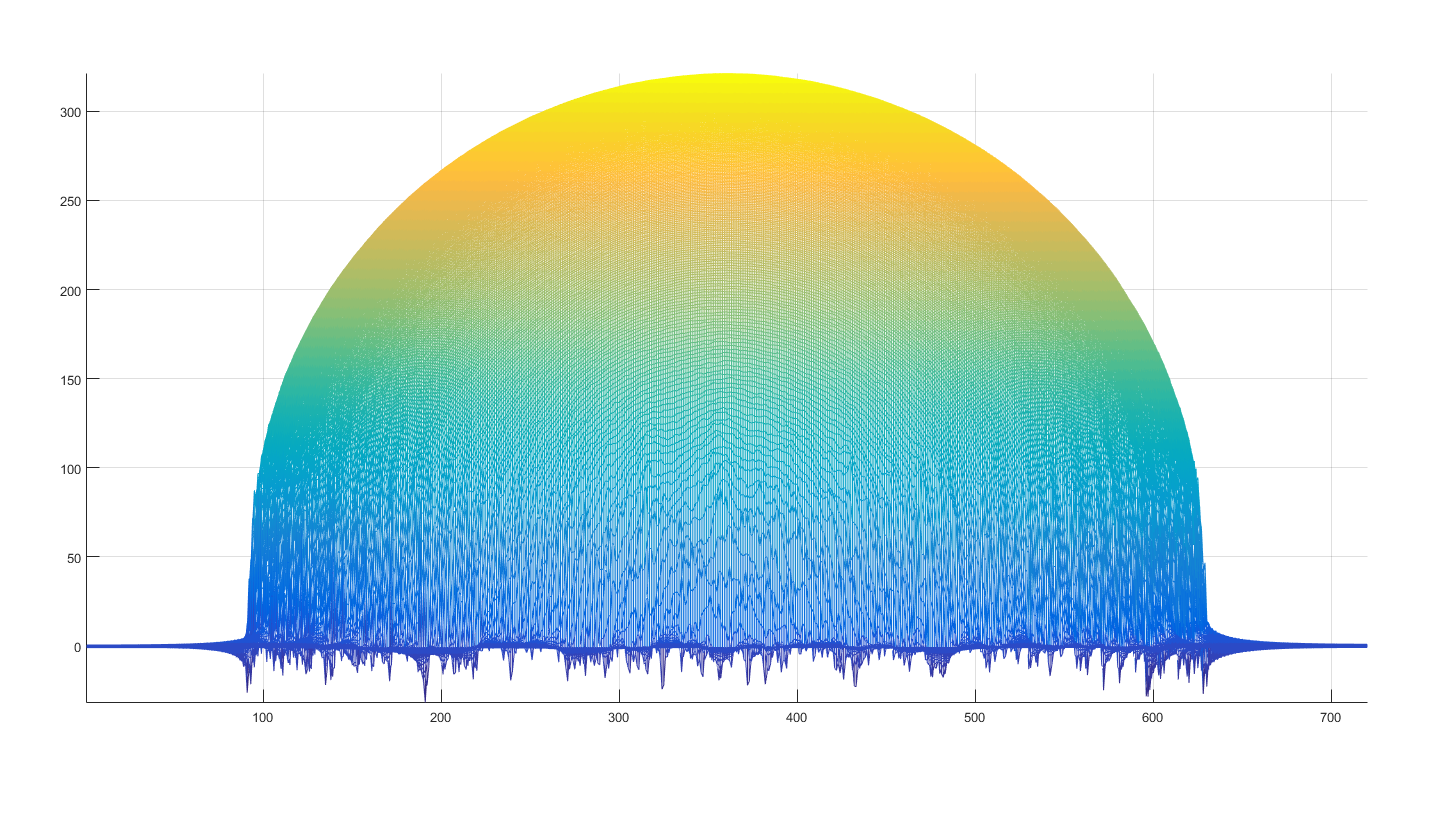
\includegraphics[width=0.33\textwidth]{mapping/ps_criteria/mu_med_5_5.png} &
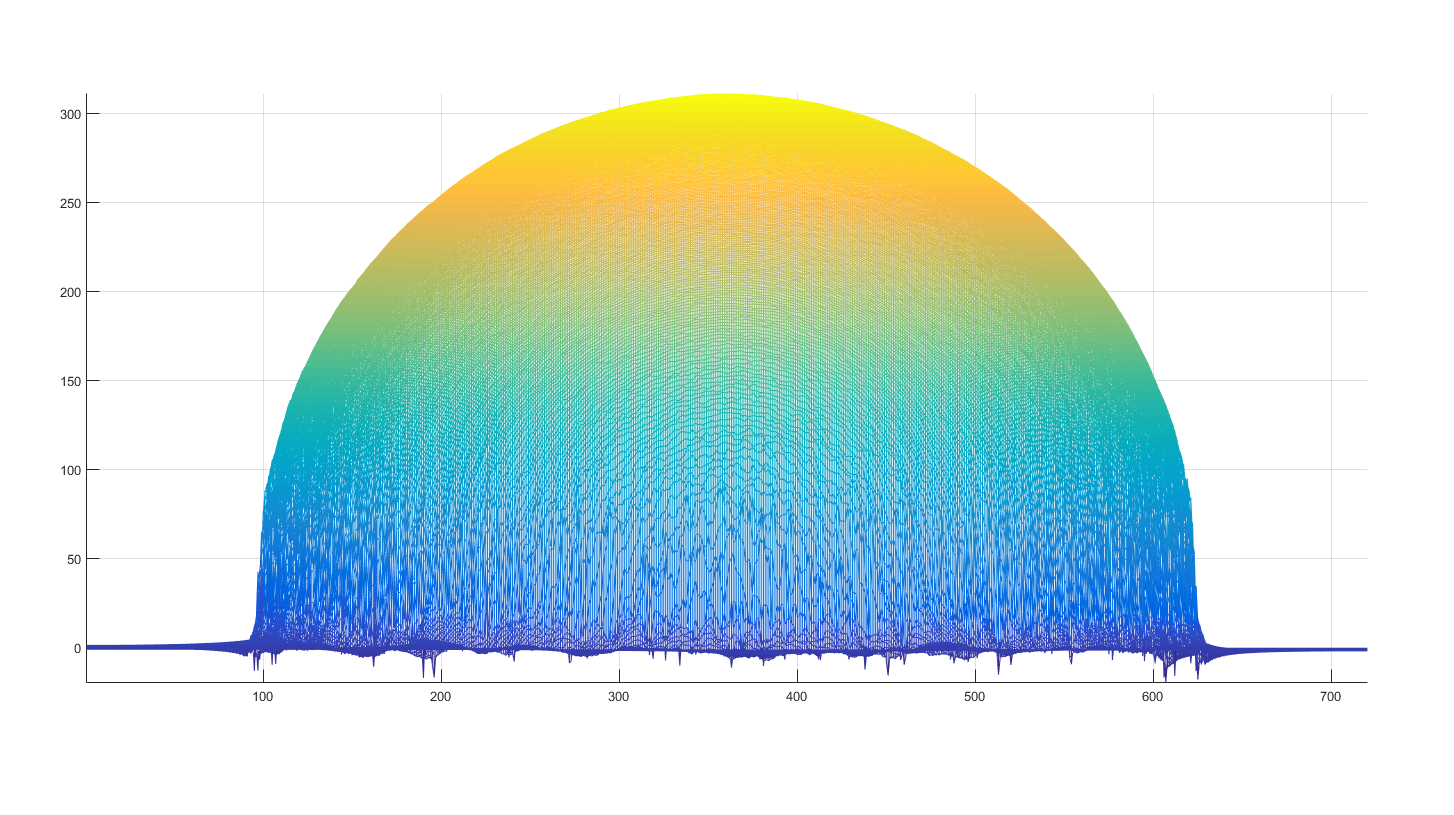
\includegraphics[width=0.33\textwidth]{mapping/ps_criteria/mu_med_10_10.png} \\
(a) $\mu=0, \text{med}=0$ & (b) $\mu=5, \text{med}=5$ & (c) $\mu=10, \text{med}=10$\\
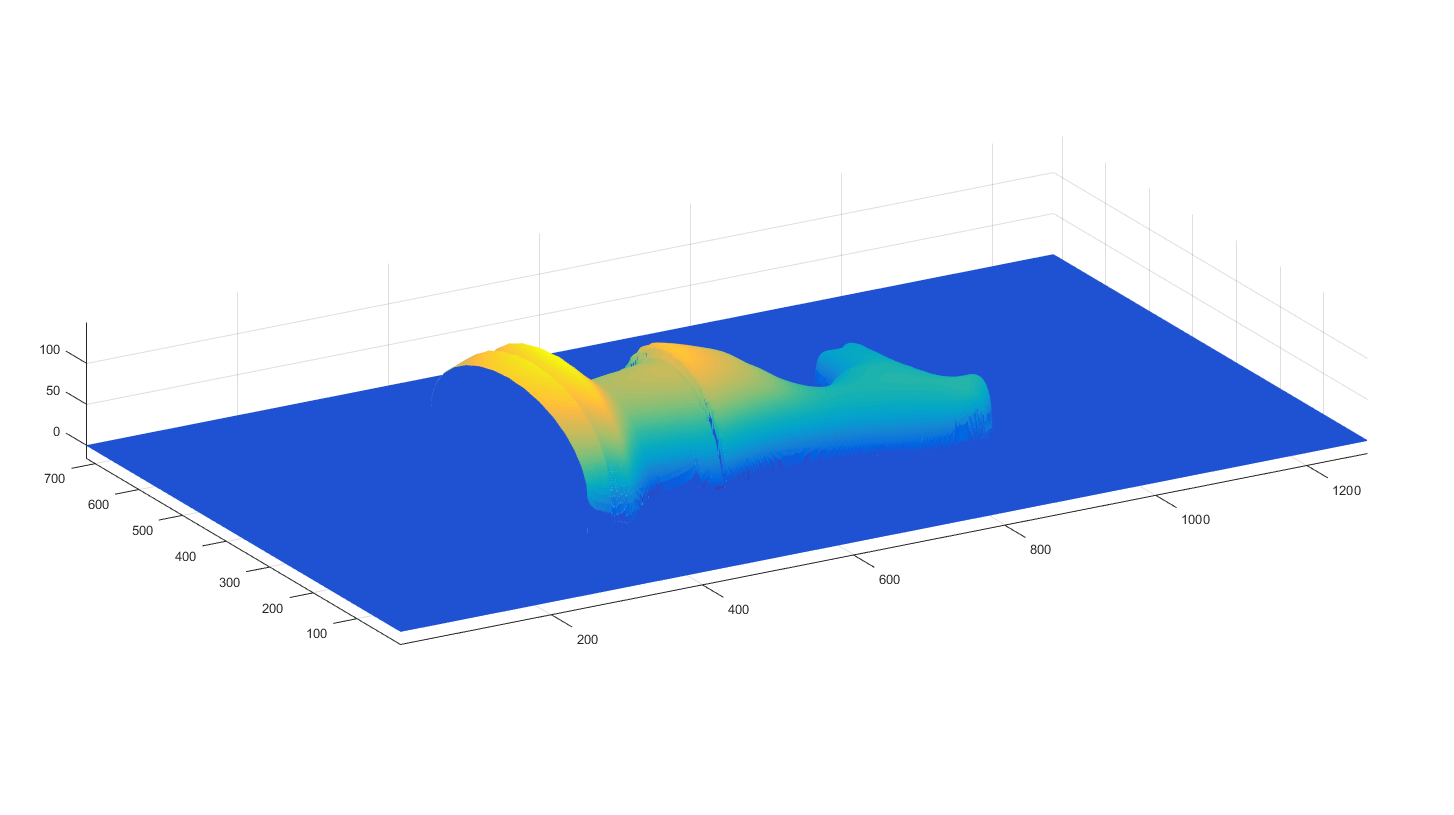
\includegraphics[width=0.33\textwidth]{mapping/ps_criteria/knight_0_0.png} &
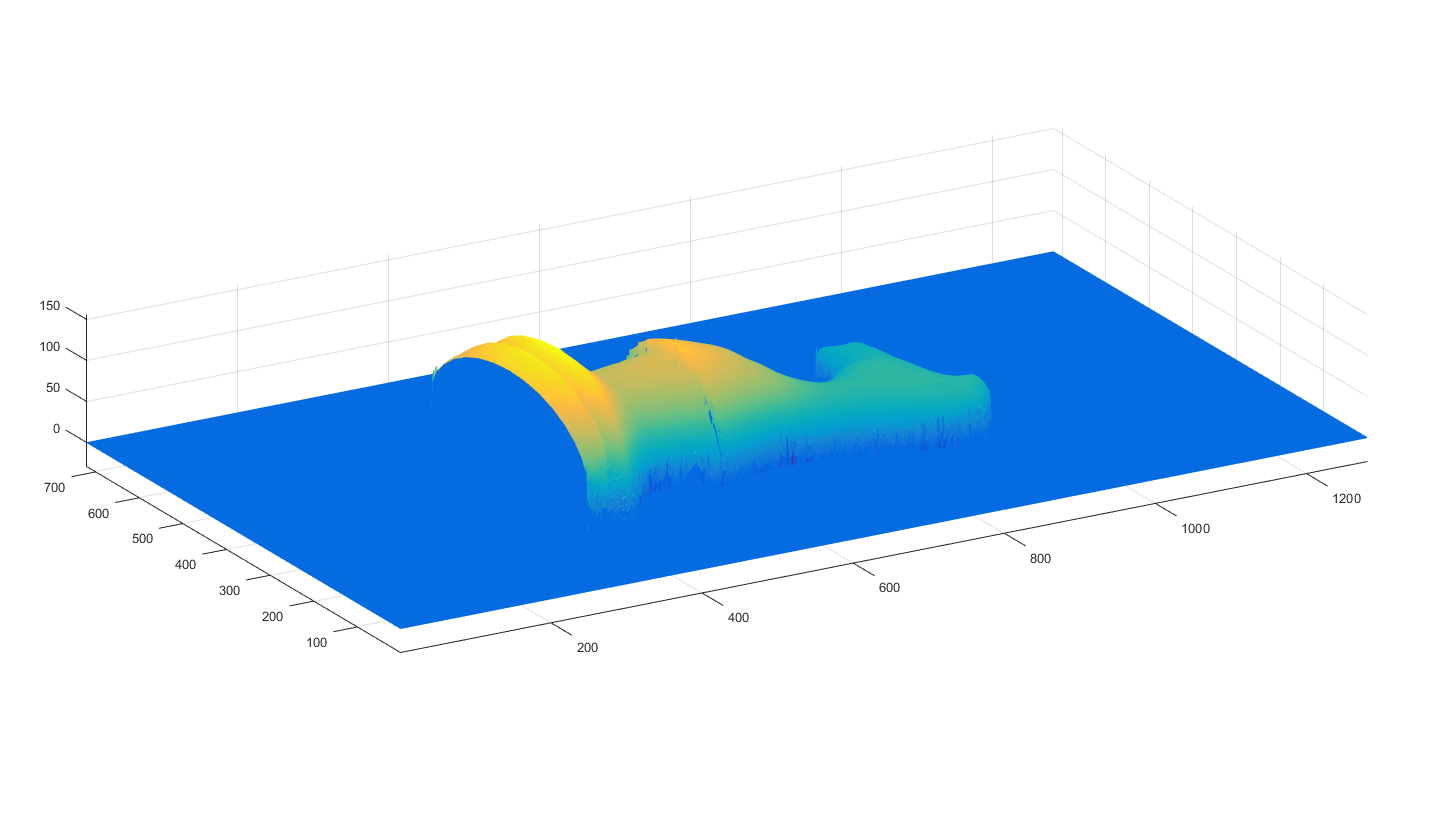
\includegraphics[width=0.33\textwidth]{mapping/ps_criteria/knight_5_5.png} &
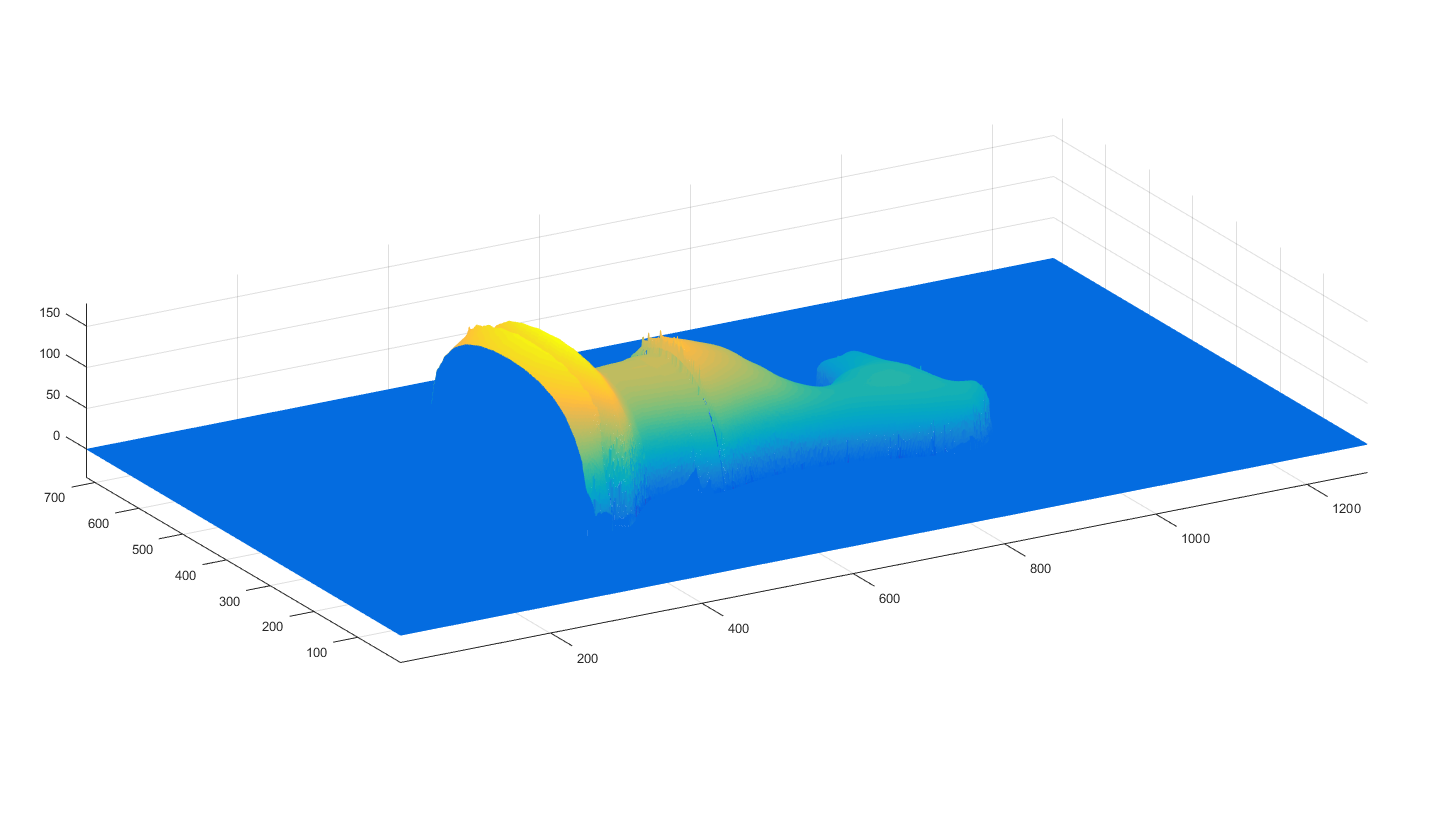
\includegraphics[width=0.33\textwidth]{mapping/ps_criteria/knight_10_10.png} \\
(d) $\mu=0, \text{med}=0$ & (e) $\mu=5, \text{med}=5$ & (f) $\mu=10, \text{med}=10$\\
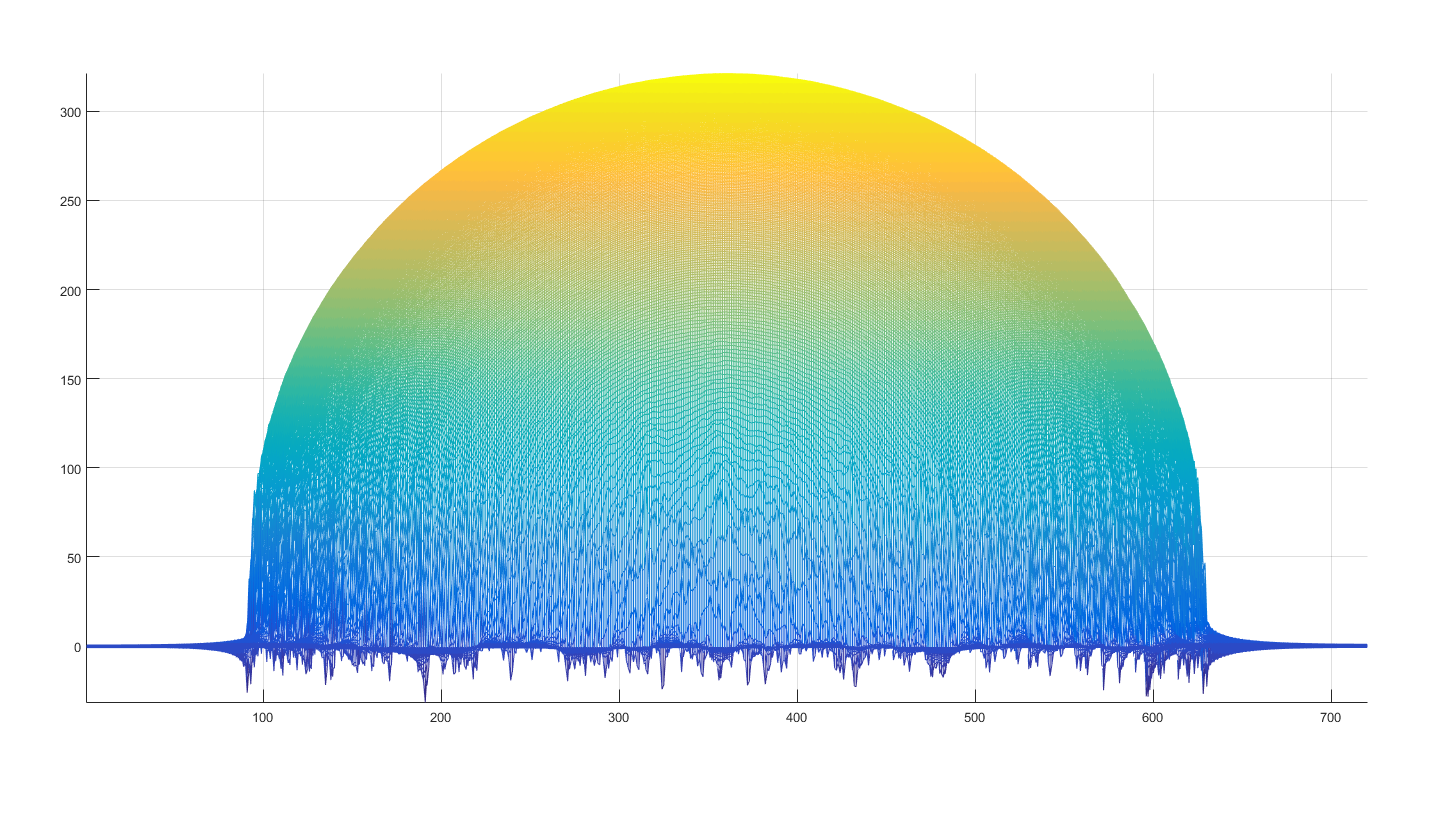
\includegraphics[width=0.33\textwidth]{mapping/ps_criteria/mu_med_5_5.png} &
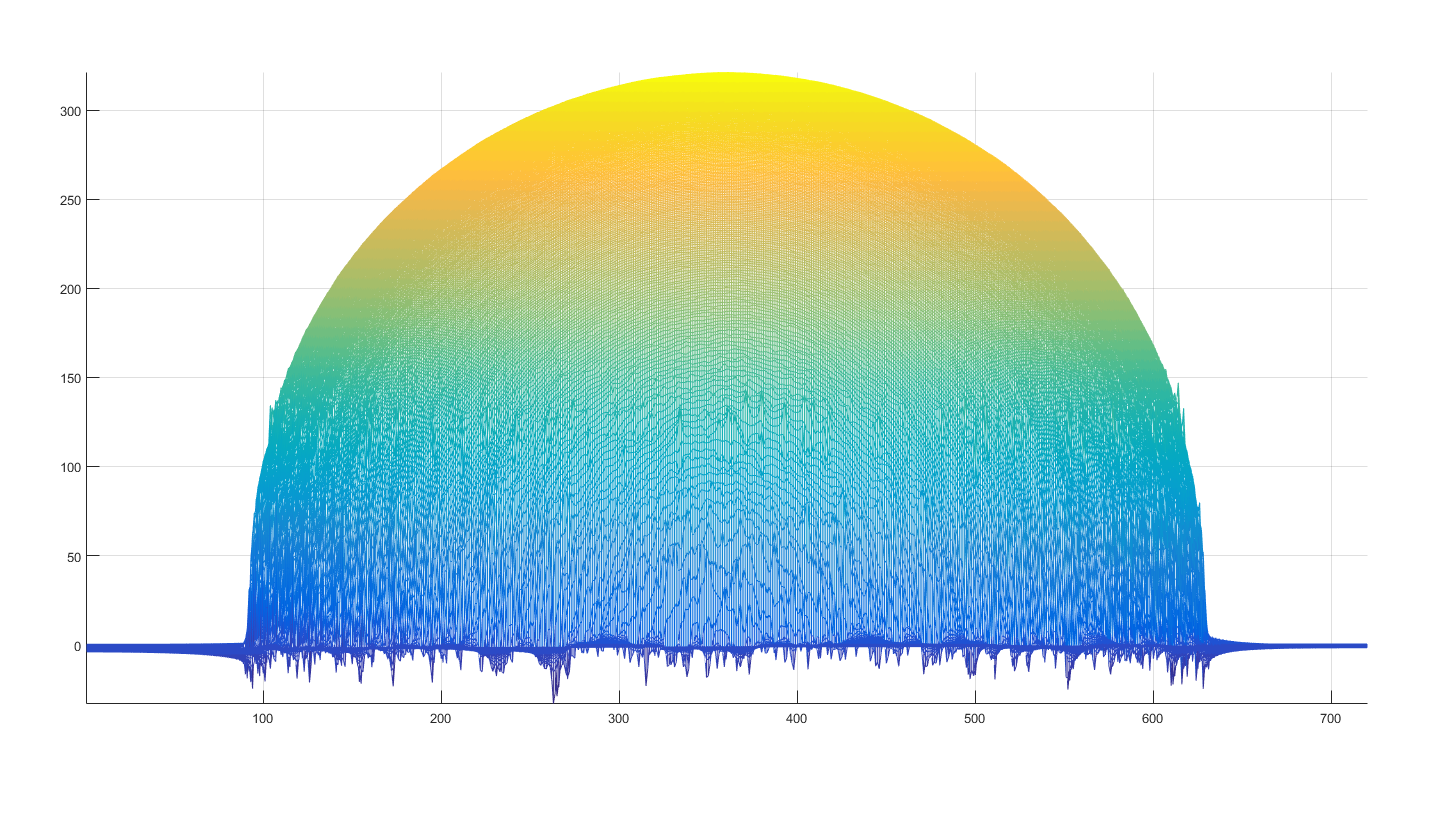
\includegraphics[width=0.33\textwidth]{mapping/ps_criteria/mu_med_5_6.png} &
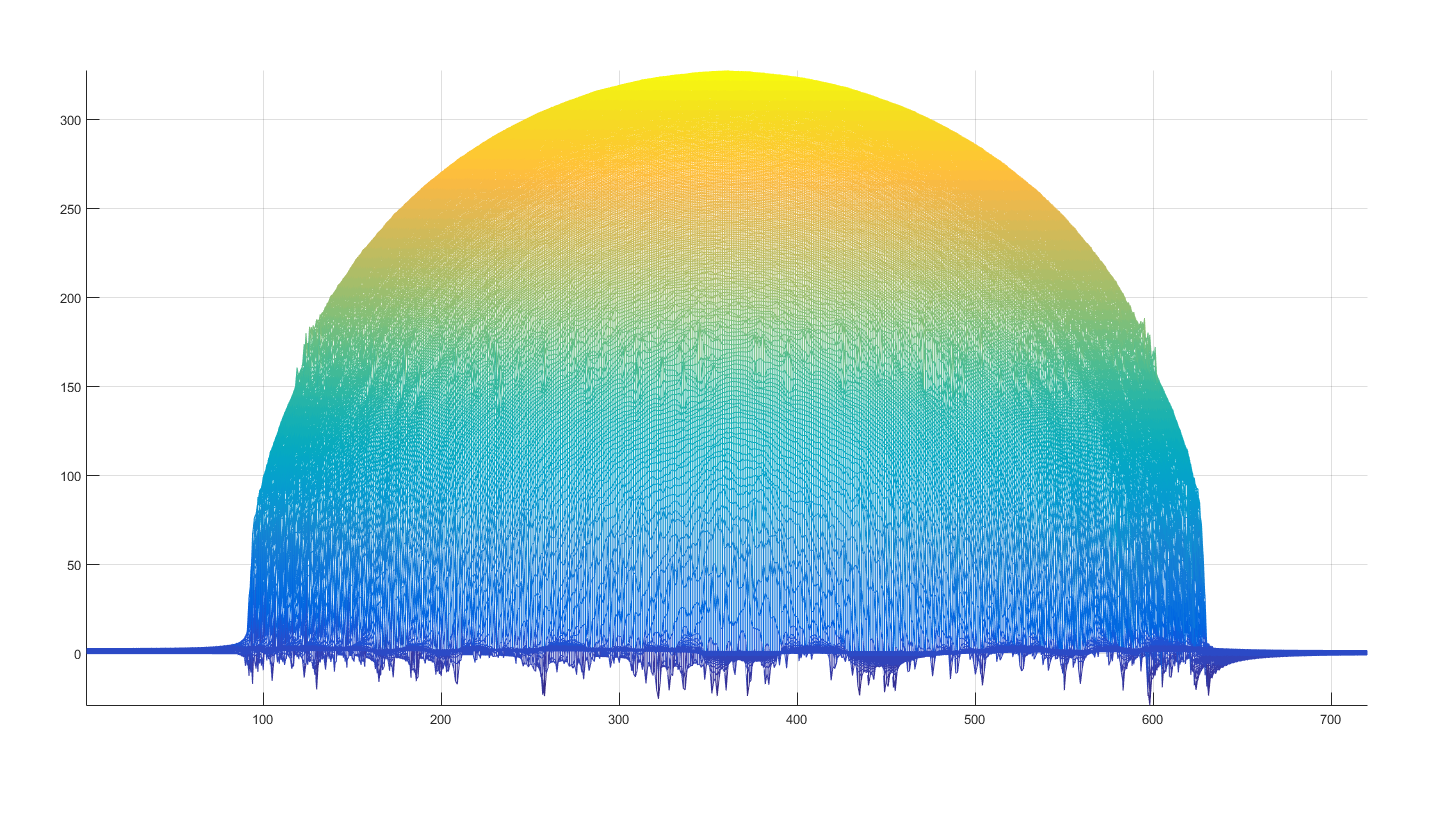
\includegraphics[width=0.33\textwidth]{mapping/ps_criteria/mu_med_5_7.png} \\
(g) $\mu=5, \text{med}=5$ & (h) $\mu=5, \text{med}=6$ & (i) $\mu=5, \text{med}=7$\\
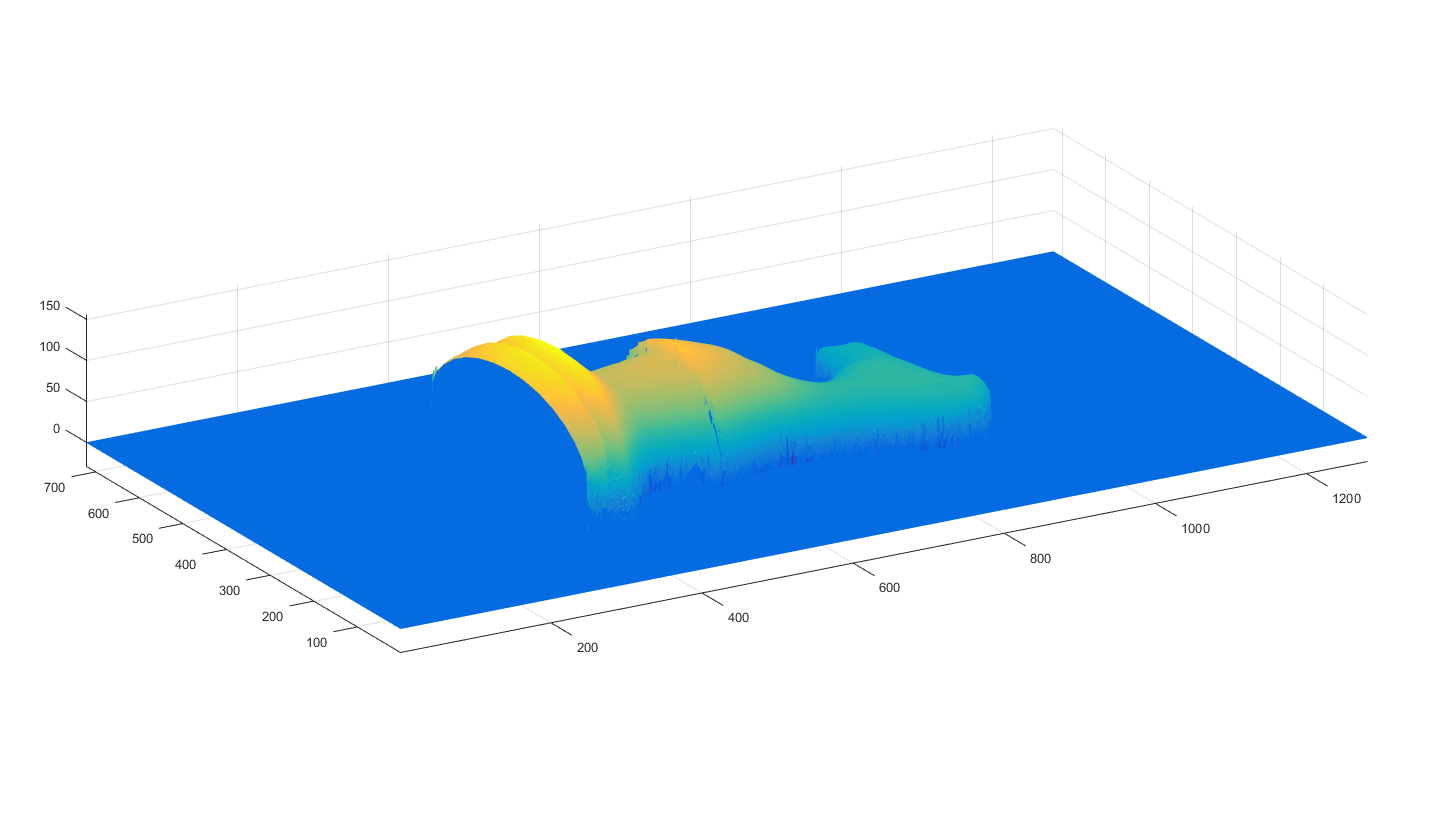
\includegraphics[width=0.33\textwidth]{mapping/ps_criteria/knight_5_5.png} &
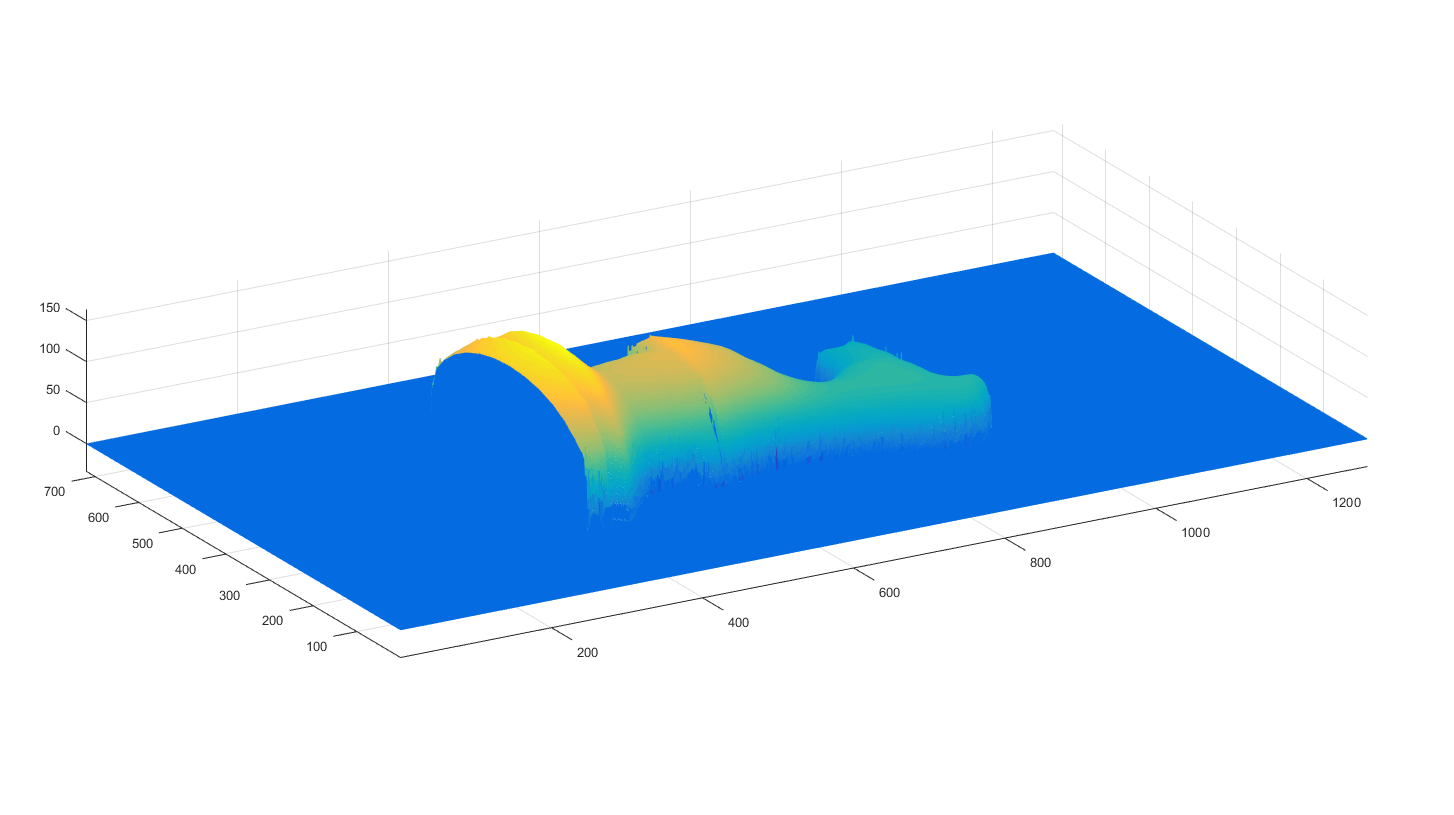
\includegraphics[width=0.33\textwidth]{mapping/ps_criteria/knight_5_6.png} &
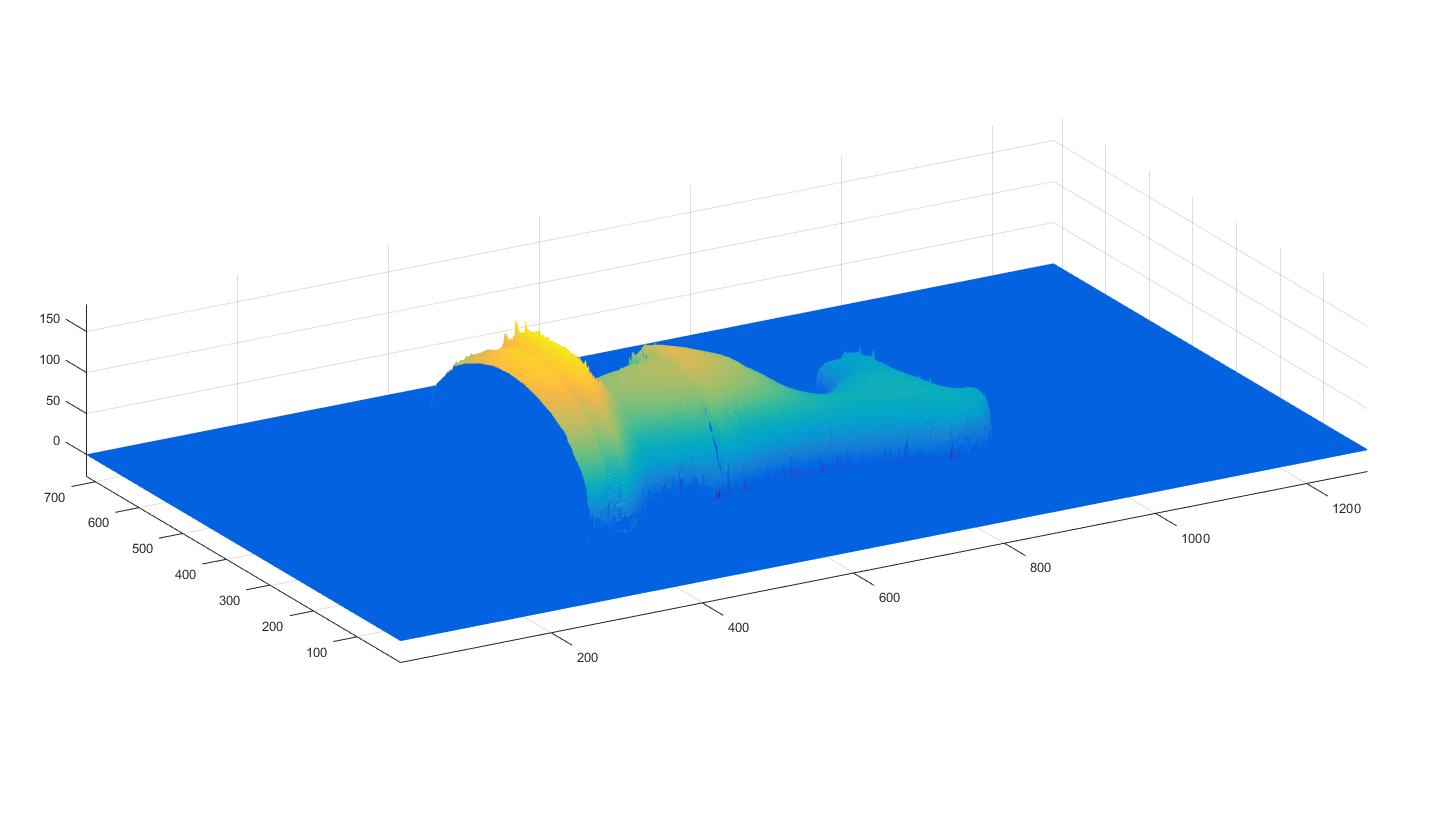
\includegraphics[width=0.33\textwidth]{mapping/ps_criteria/knight_5_8.png} \\
(j) $\mu=5, \text{med}=5$ & (k) $\mu=5, \text{med}=6$ & (l) $\mu=5, \text{med}=8$\\
\end{tabular}
\caption{Shape estimation results with varied mean and median values. The algorithm is less sensitive to large mean or median value while more sensitive to the difference between the mean and median value.}
\label{fig:ps_criteria}
\end{figure}

% However, as we will be shown in Chapter~\ref{ch:3DRecon_Interp}, the actual thresholds of the angular error might vary from shape to shape. Therefore, it's impractical to use a categorical numeric value to determine the quality of reconstruction. The metrics mentioned above provide the guidelines when it comes to assess the performance of the algorithm, but the actual thresholds are by no means and should not be fixed.

% Therefore, the criteria of an ``acceptable'' normal reconstruction are listed in Table~\ref{tab:ps_criteria}, where $c$ is a constant that varies from object to object, and is normally less then $5^\circ$. For the examples shown in Figure~\ref{fig:ps_criteria}, $c=1^\circ$ for sphere, and $c=2^\circ$ for `knight'.
% \begin{table}[!htbp]
% \centering
% \begin{tabular}{cccc}
% \hline
% Mean ($\mu$) & Median (med) & Interquatile & Standard Deviation\\
% \hline
% $\mu<10^\circ$ & $\text{med}<10^\circ$ & $Q_{(3-1)}<3^\circ$ & $\sigma \not\gg Q_3$\\
% $\mu - \text{med} < \text{c}^\circ$\\
% \hline
% \end{tabular}
% \caption{Criteria of an ``acceptable'' normal estimation by Photometric Stereo techniques.}
% \label{tab:ps_criteria}
% \end{table}

\section{Effective Problem Domain}
The biggest challenge in conducting a comprehensive evaluation is the large variations in shapes and material properties, which results in a problem domain that is too large to cope with. Therefore, the first step is to establish the \textit{effective problem domain} (EPD) by finding the effective properties so that the dimension of the problem conditions would become more manageable. We conduct comprehensive experiments that evaluate the performance of the algorithms by changing two properties at a time while fixing the others. The goals are to 1). identify effective properties; 2). identify dependent properties that would impact the algorithm differently with different combinations of values.

\subsection{EPD of PMVS}
We evaluate the performance of PMVS in terms of accuracy and completeness under varied combinations of properties, the settings of the properties are listed in Table~\ref{tab:mvs_depend_check_params}.
\begin{table}[!htbp]
  \centering
  \begin{tabular}{l*{4}{c}}
  \hline
  \textbf{Group} & Texture & Albedo & Specular & Roughness\\
  \hline
  \textbf{(a)} & [0.2, 0.8] & [0.2, 0.8] & 0.0 & 0.0\\
  \textbf{(b)} & [0.2, 0.8] & 0.8 & [0.2, 0.8] & 0.0\\
  \textbf{(c)} & [0.2, 0.8] & 0.8 & 0.0 & [0.2, 0.8]\\
  \textbf{(d)} & 0.8 & [0.2, 0.8] & [0.2, 0.8] & 0.0\\
  \textbf{(e)} & 0.8 & [0.2, 0.8] & 0.0 & [0.2, 0.8]\\
  \textbf{(f)} & 0.8 & 0.8 & [0.2, 0.8] & [0.2, 0.8]\\
  \hline
  \end{tabular}
  \caption{Problem conditions for establishing the \textit{effective problem domain} of PMVS.}
  \label{tab:mvs_depend_check_params}
\end{table}

\begin{sidewaysfigure}[!htbp]
\begin{tabular}{ccc}
\includegraphics[width=0.3\textwidth]{mapping/depend_check/mvs_tex_alb}&
\includegraphics[width=0.3\textwidth]{mapping/depend_check/mvs_tex_spec}&
\includegraphics[width=0.3\textwidth]{mapping/depend_check/mvs_tex_rough}\\
(a) & (b) & (c)\\
\includegraphics[width=0.3\textwidth]{mapping/depend_check/mvs_alb_spec}&
\includegraphics[width=0.3\textwidth]{mapping/depend_check/mvs_alb_rough}&
\includegraphics[width=0.3\textwidth]{mapping/depend_check/mvs_spec_rough}\\
(d) & (e) & (f)\\
\end{tabular}
\caption{Performance of PMVS under six pairwise conditions. For instance, (a) shows the performance under changing \textit{texture} and \textit{albedo} values while the others are fixed. The property values are set based on settings in Table~\ref{tab:mvs_depend_check_params}.}
\label{fig:mvs_depend_check}
\end{sidewaysfigure}

\subsubsection{Effective and Dependent Properties}
We investigate how each property affects the reconstruction in terms of accuracy and completeness.

\textbf{(a) Texture and Albedo} 
The texture has a positive effect on the reconstruction in terms of accuracy and completeness while the effect of albedo is negligible.

\textbf{(b) Texture and Specular} 
Specular has a negative effect on both the accuracy and completeness of the reconstruction. However, the level of impact varies as the texture varies, more specifically, the effect of specular is more substantial on a lower textured surface than that on a higher textured one. This could be explained as follows: the specular lobe can only be observed by cameras positioned and oriented towards the specular lobe, such as the camera $V_2$ shown in Figure~\ref{fig:mvs_spec} (a) and (c). Cameras positioned otherwise would observed the true surface, such as camera $V_1$ shown in Figure~\ref{fig:mvs_spec} (a) and (b). The algorithm would exploit the texture information provided by views like $V_1$, and thus is able to reconstruct a specular surface.
\begin{figure}[!htbp]
\begin{tabular}{ccc}
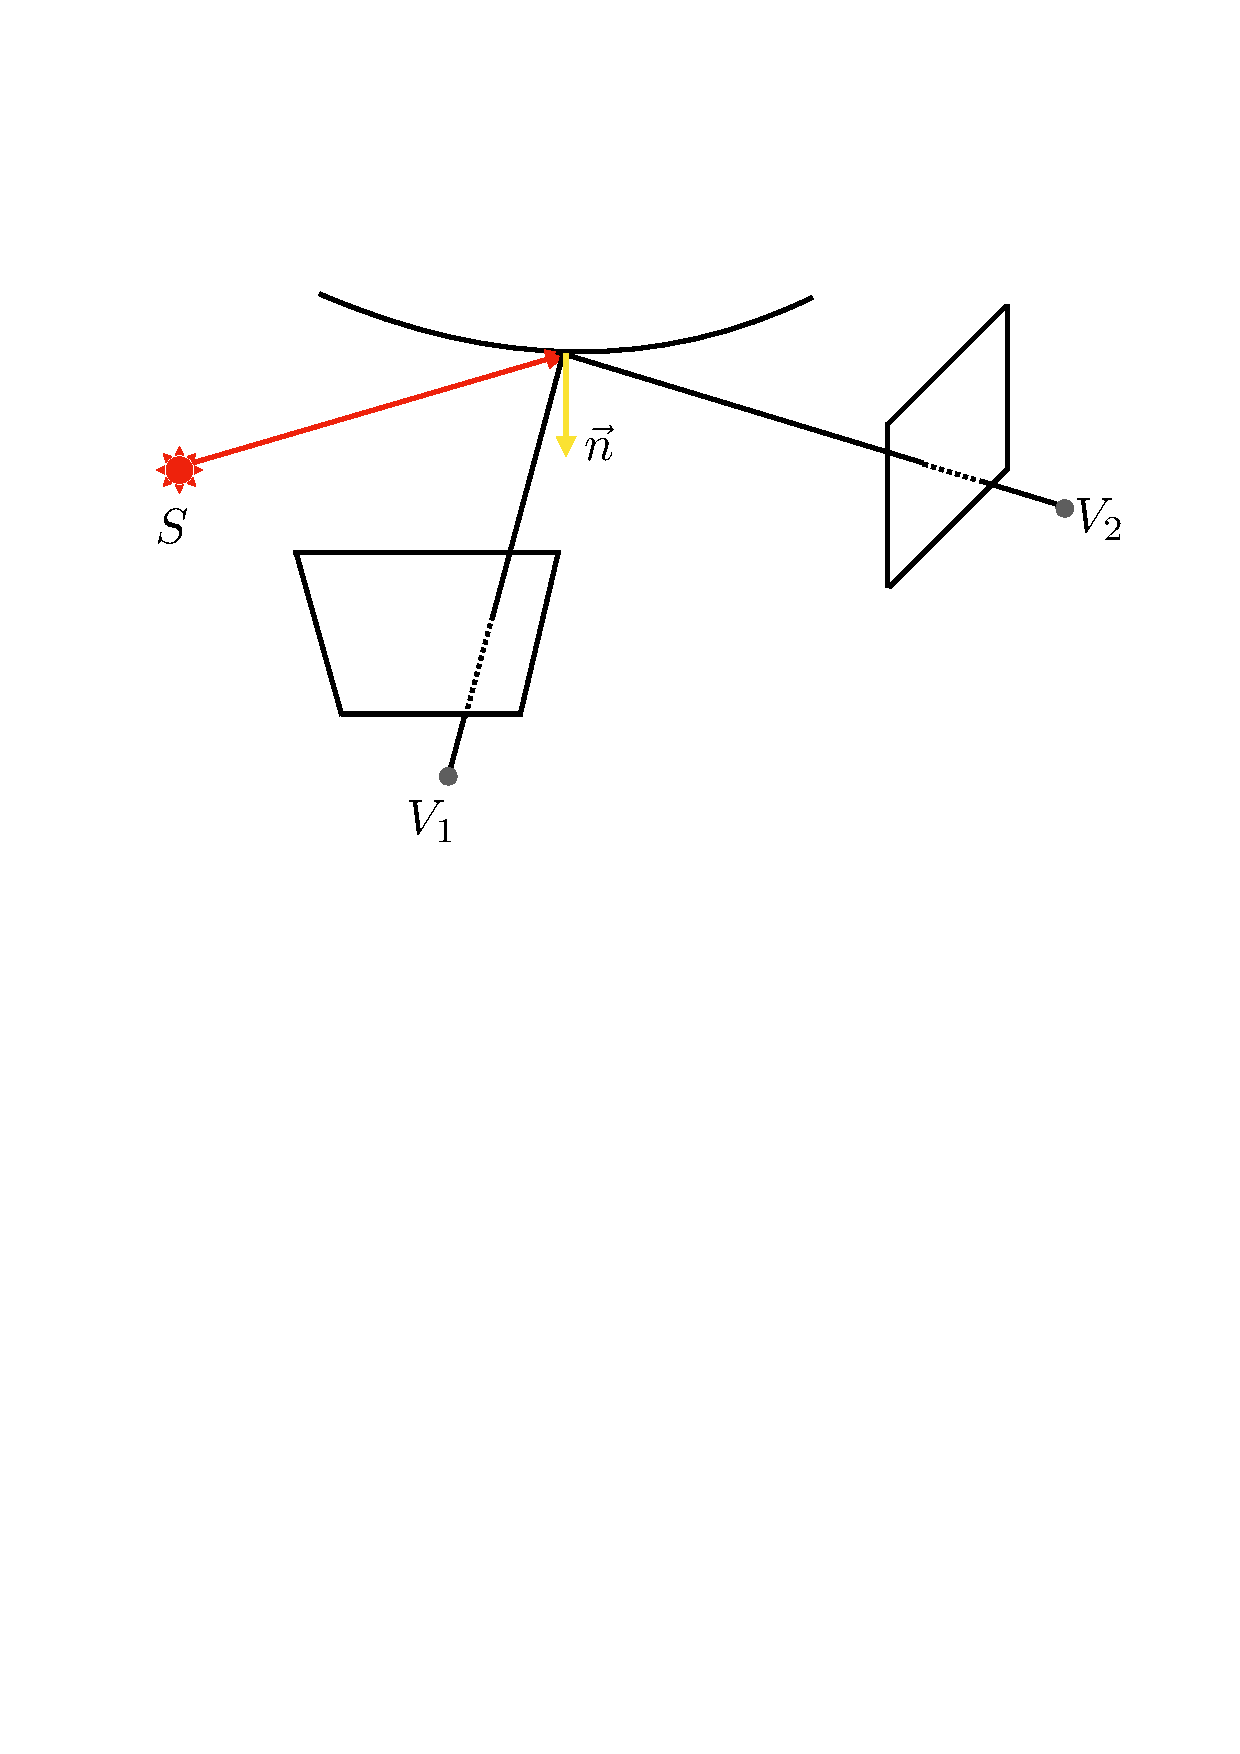
\includegraphics[width=0.33\textwidth]{mapping/mvs_spec/mvs_spec}&
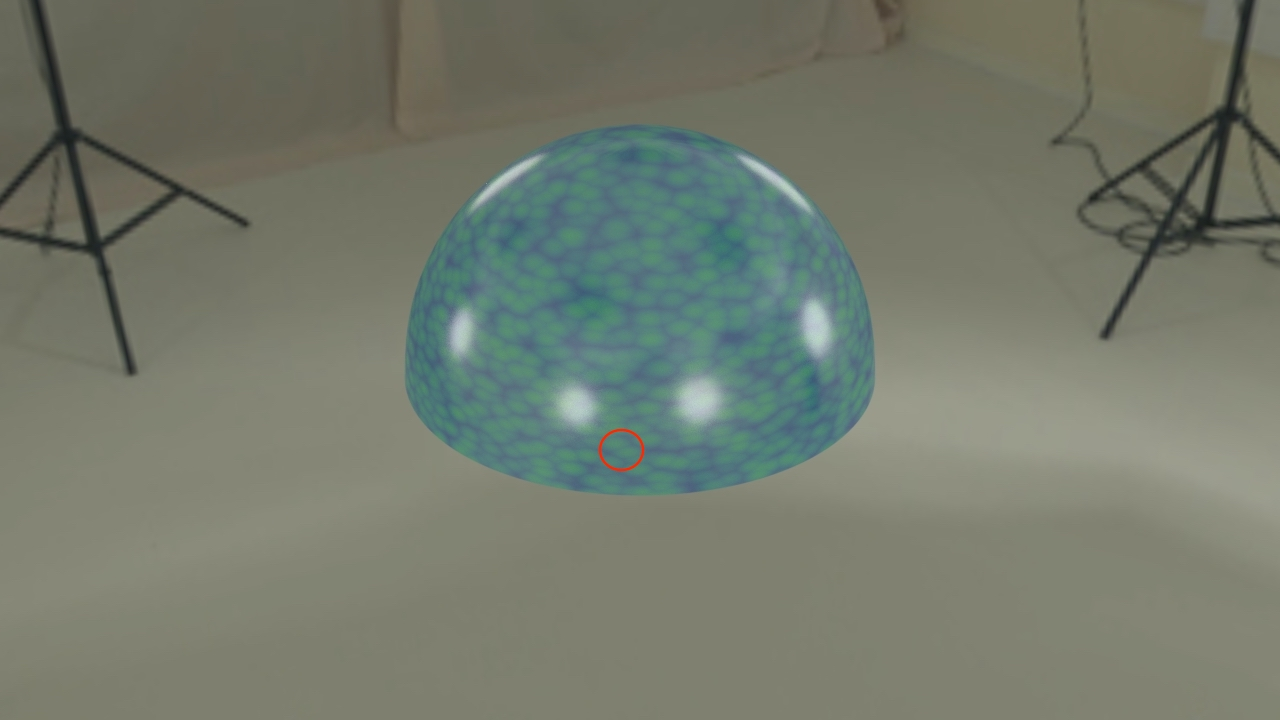
\includegraphics[width=0.33\textwidth]{mapping/mvs_spec/mvs_spec_01}&
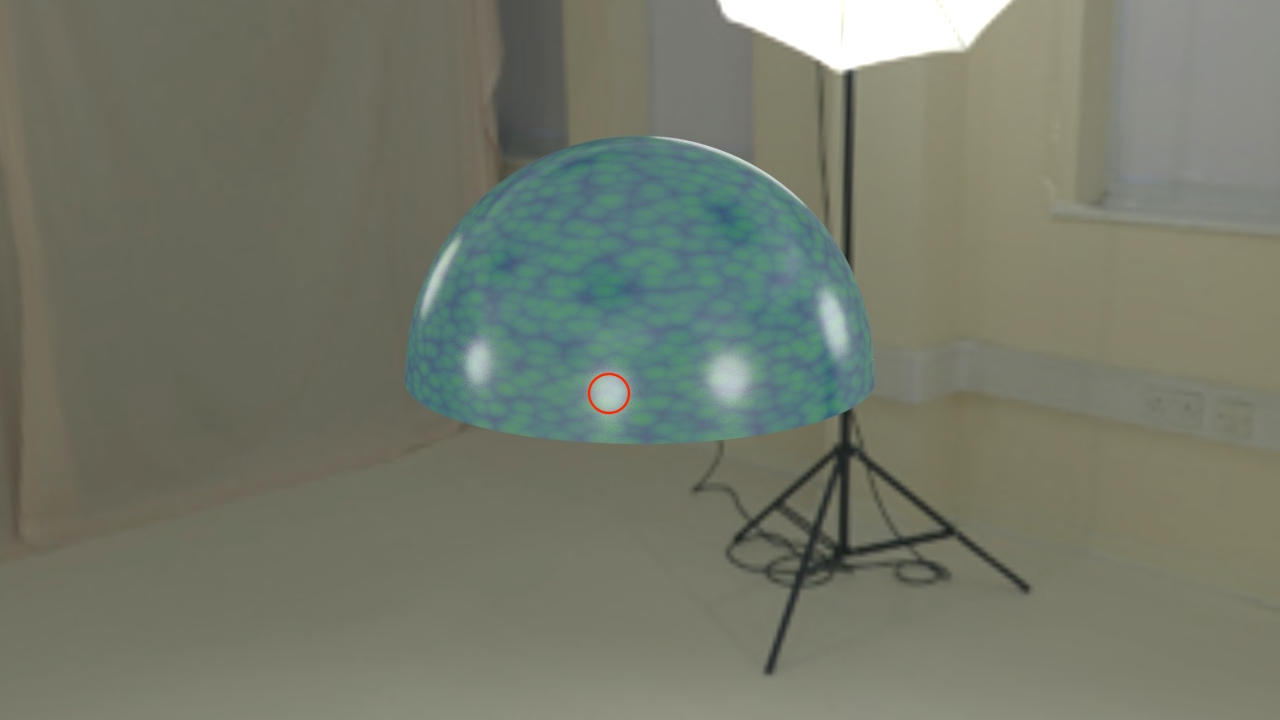
\includegraphics[width=0.33\textwidth]{mapping/mvs_spec/mvs_spec_00}\\
(a) Image formation & (b) $V_1$ & (c) $V_2$\\
\end{tabular}
\caption{(a) shows the reflection of light off a specular surface. $V_1$ received the diffuse component while $V_2$ receives the specular component. (b), (c) shows the images observed from these two views. The specular area (red circle) observed in $V_2$ is visible in $V_1$.}
\label{fig:mvs_spec}
\end{figure}

\textbf{(c) Texture and Roughness} 
Roughness doesn't have a significant effect on the results.

\textbf{(d) Albedo and Specular} 
Albedo has a positive effect whereas specular a negative effect on the reconstruction. Furthermore, the effect of specular is far more substantial on a lower albedo surface than that on a higher albedo one. This can be explained as follows: according to the energy conservation law, as the specular component increases, the diffuse component decreases, thus the diffuse area becomes less discernible, see Figure~\ref{fig:mvs_alb_spec} (a)-(c). Increasing the diffuse albedo can counteract the effect of specular and make the texture visible again, see Figure~\ref{fig:mvs_alb_spec} (d)-(f).
\begin{figure}[!htbp]
\centering
\begin{tabular}{ccc}
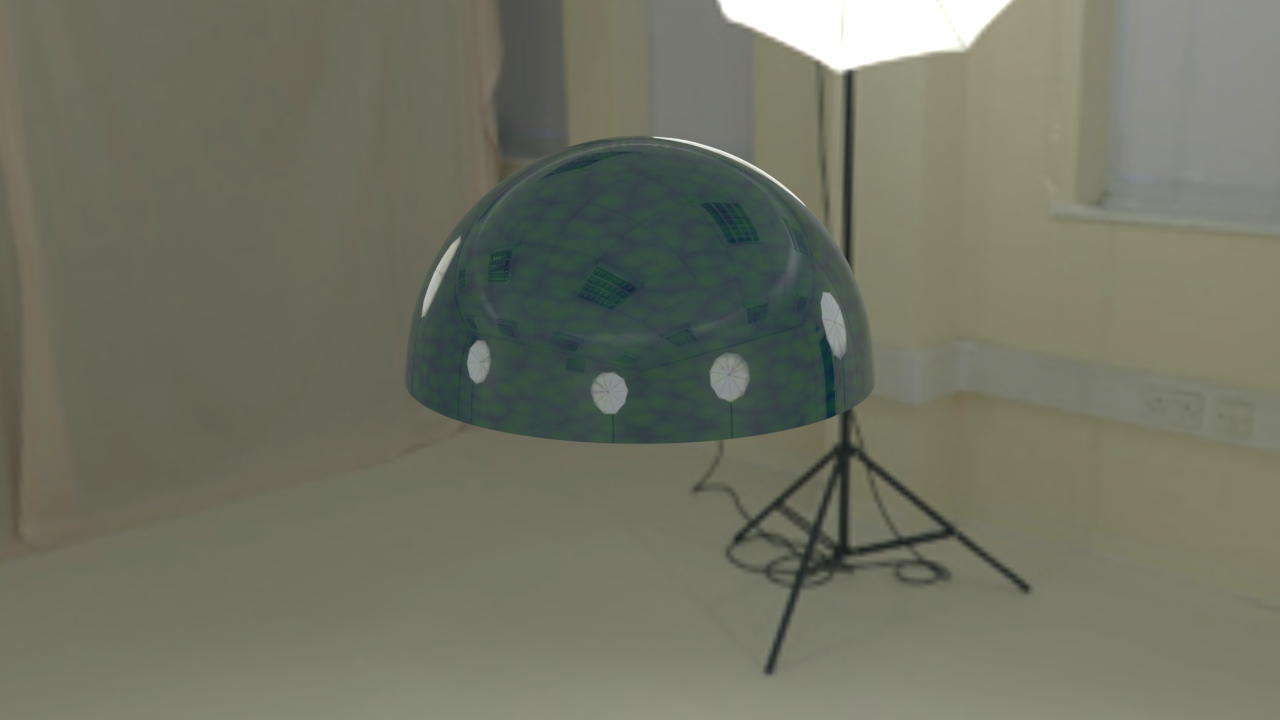
\includegraphics[width=0.33\textwidth]{mapping/mvs_alb_spec/alb_spec_0202}&
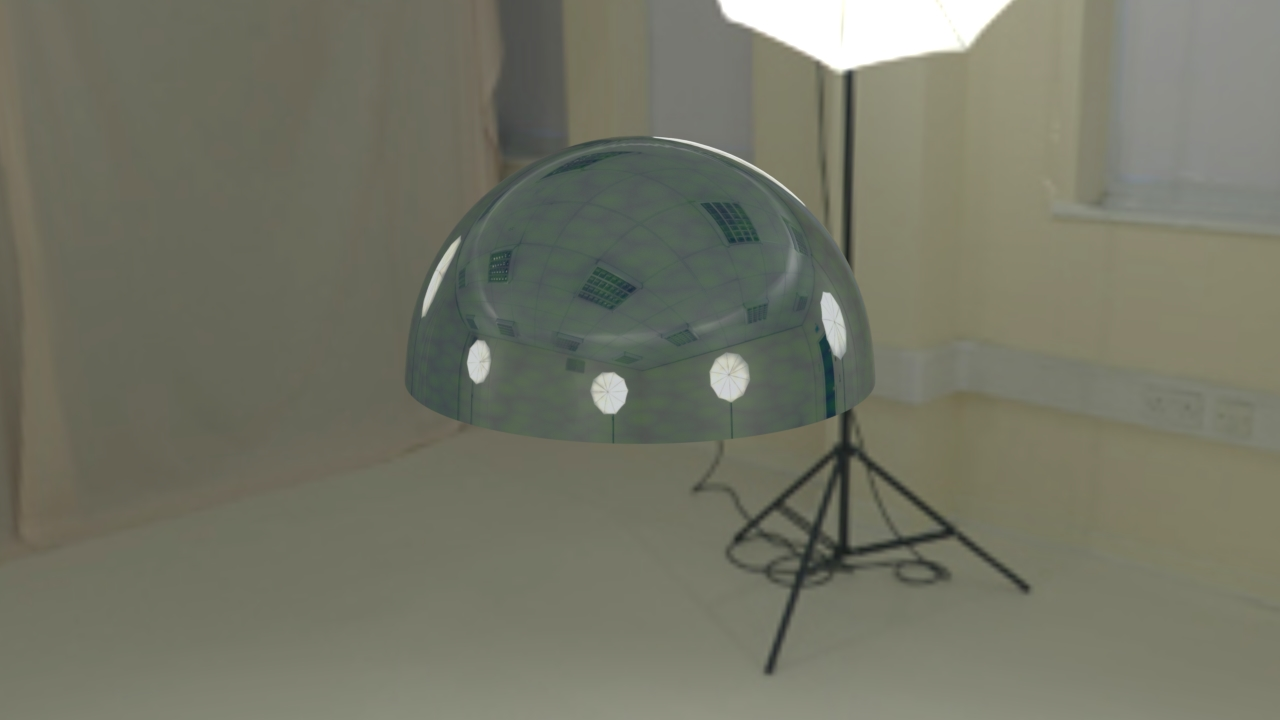
\includegraphics[width=0.33\textwidth]{mapping/mvs_alb_spec/alb_spec_0205}&
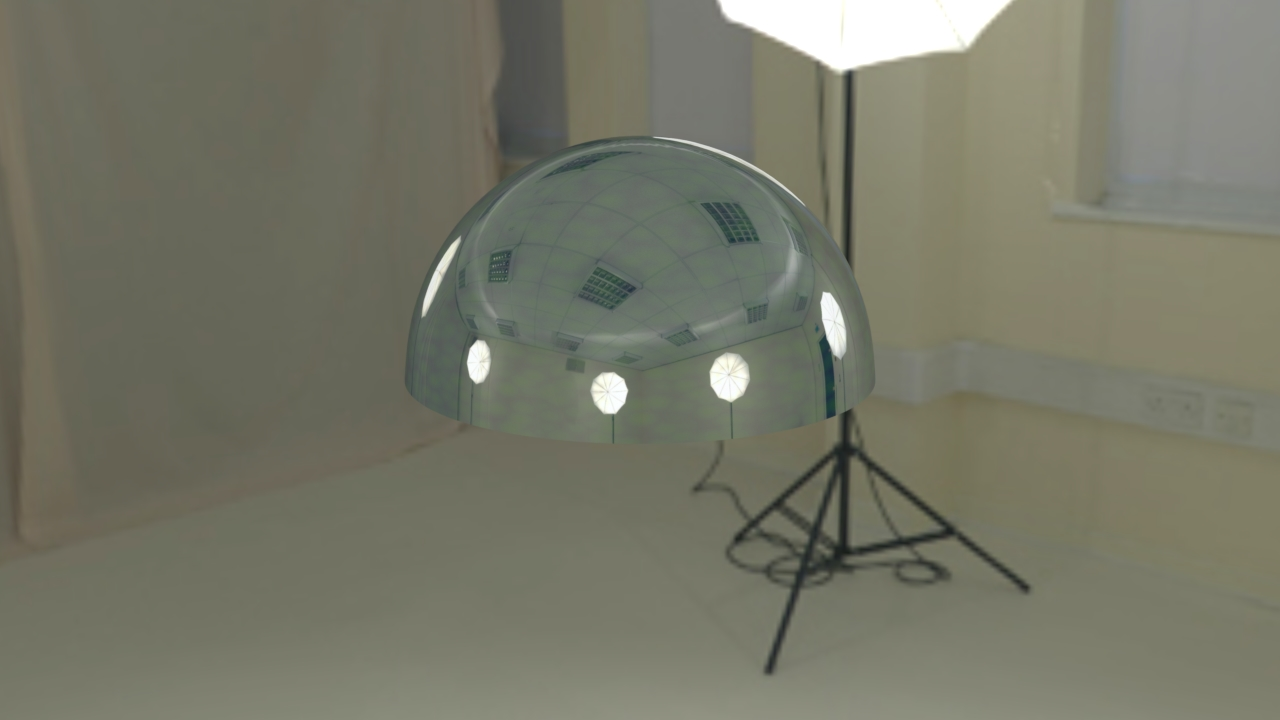
\includegraphics[width=0.33\textwidth]{mapping/mvs_alb_spec/alb_spec_0208}\\
(a) spec: 0.2 & (b) spec: 0.5 & (c) spec: 0.8\\
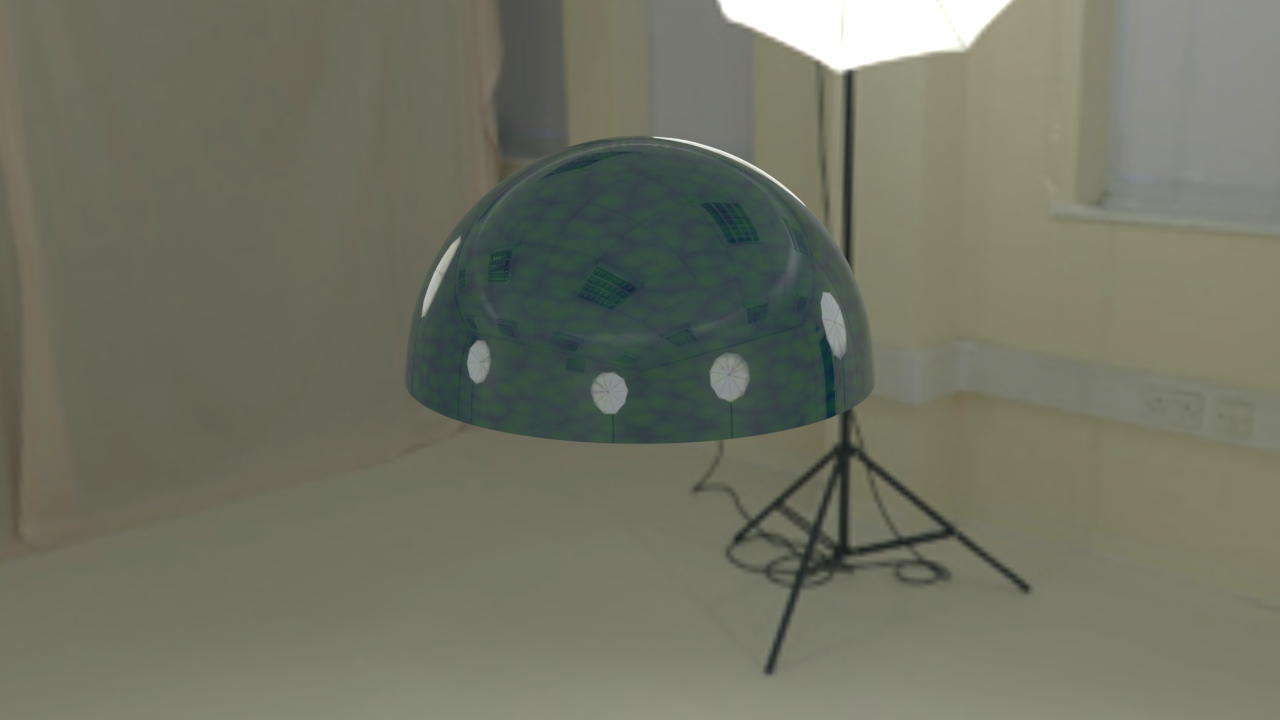
\includegraphics[width=0.33\textwidth]{mapping/mvs_alb_spec/alb_spec_0202}&
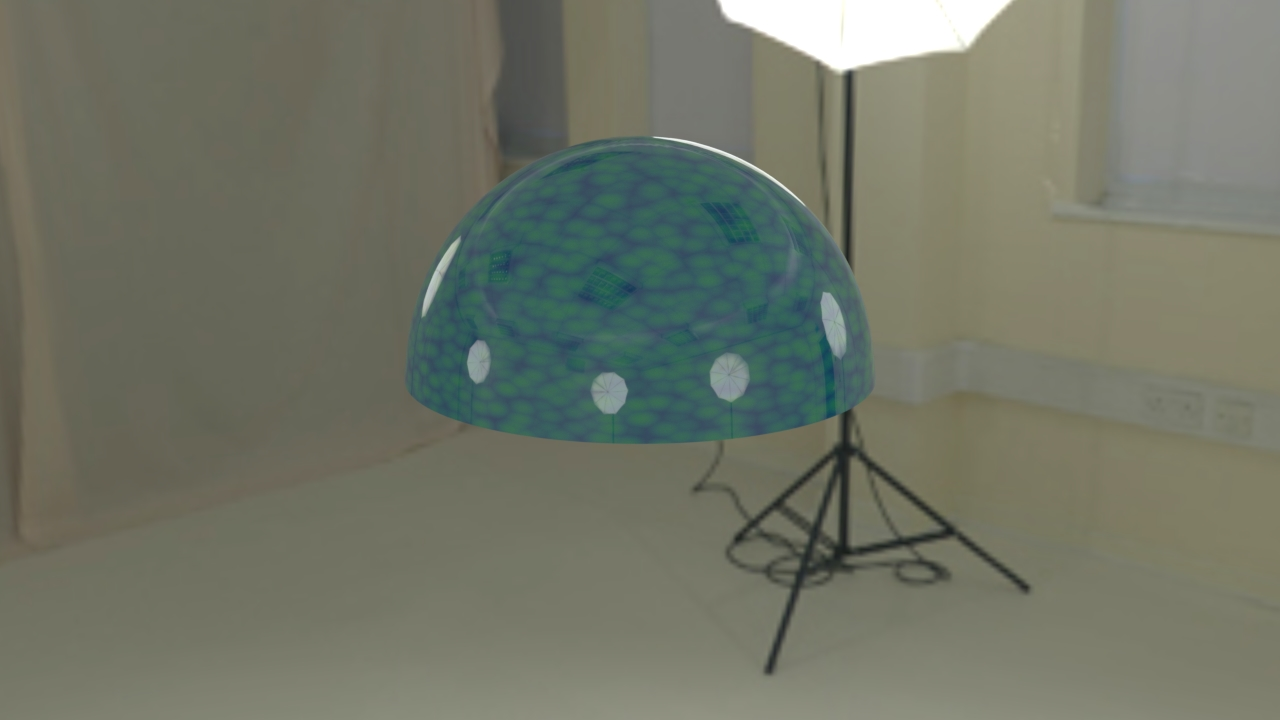
\includegraphics[width=0.33\textwidth]{mapping/mvs_alb_spec/alb_spec_0502}&
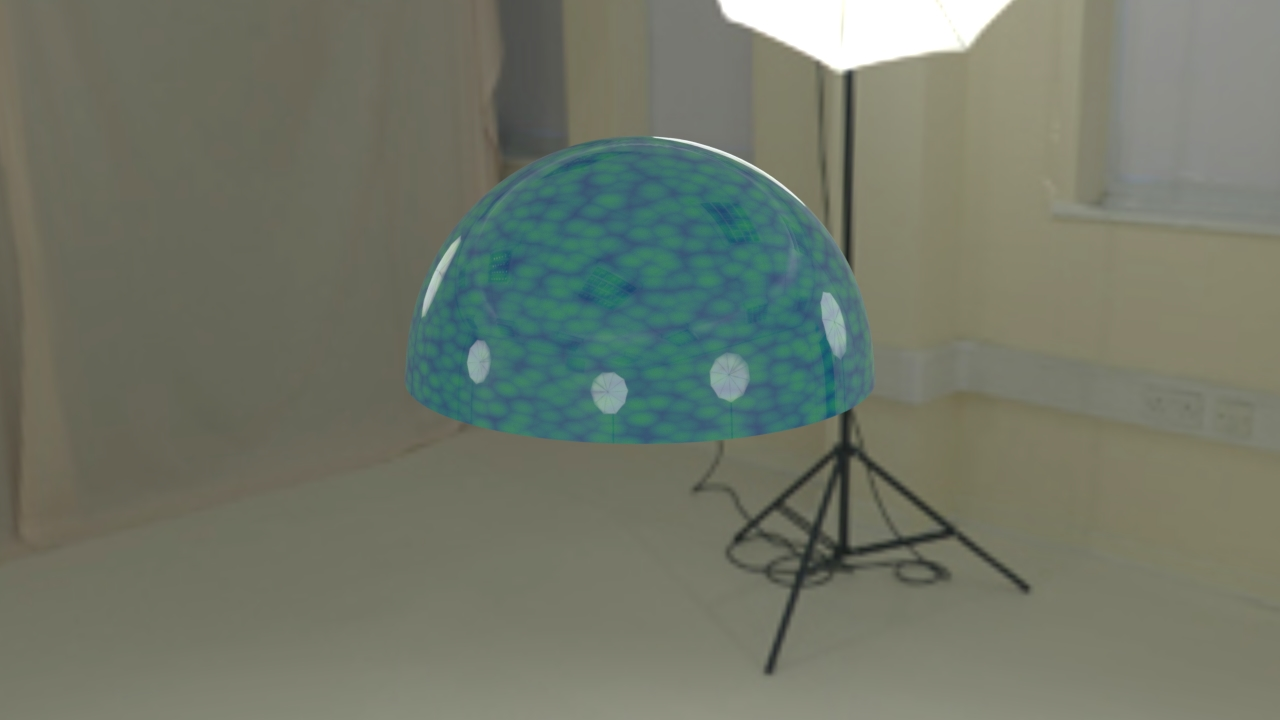
\includegraphics[width=0.33\textwidth]{mapping/mvs_alb_spec/alb_spec_0802}\\
(d) alb: 0.2 & (e) alb: 0.5 & (f) alb: 0.8\\
\end{tabular}
\caption{(a)-(c). The albedo is set as 0.2, (d)-(f). the specular is set as 0.2. According to energy conservation, as the specular component increases, the diffuse component decreases.}
\label{fig:mvs_alb_spec}
\end{figure}

\textbf{(e) Albedo and Roughness}
The albedo and roughness have a negligible effect on the results.

\textbf{(f) Specular and Roughness} 
Surface roughness can effectively diminishes the specular component and makes the surface appearch more diffuse. Since specular has a negative impact on the reconstruction, in theory, roughness should have a positive impact on the reconstruction. However, this effect is closely related to surface texture: surface reconstruction is always poor for low textured surfaces or good for highly textured ones regardless of the amount of specular component, as shown in Figure~\ref{fig:mvs_depend_check} (b). The result shown in Figure~\ref{fig:mvs_depend_check} (f) happens to be tested in highly textured surface, therefore achieves consistently good results. Since high specular, high roughness surfaces visually resemble low specular ones, and achieve similar reconstruction results as well, we would only consider specular, and ignore roughness for simplicity.

\subsubsection{Summary} 
The effective properties of PMVS are: texture, albedo, and specular, of which texture is the most important one. Specular would deteriorate the reconstruction for lower textured and lower albedo surfaces. The effective problem domain is shown in Table~\ref{tab:mvs_depend_prop}.
\begin{table}[!htbp]
  \centering
  \begin{tabular}{l*{4}{c}}
  \hline
  \textbf{Metric} & Texture & Albedo & Specular & Roughness\\
  \hline
  Accuracy & \checkmark & \checkmark & \checkmark & \ding{55}\\
  Completeness & \checkmark & \checkmark & \checkmark & \ding{55}\\
  \hline
  \end{tabular}
  \caption{The \textit{effective problem domain} of PMVS in terms of accuracy and completeness.}
  \label{tab:mvs_depend_prop}
\end{table}

\subsection{EPD of EPS}
We evaluate the performance of example-based PS in terms of angular error under varied combinations of properties, The statistical measures that we used include median, mean, standard deviation, first and third quartile of the angular error. We investigate two properties at a time. The settings of the properties are listed in Table~\ref{tab:ps_depend_check_params}.
\begin{table}[!htbp]
  \centering
  \begin{tabular}{l*{4}{c}}
  \hline
  \textbf{Group} & Texture & Albedo & Specular & Roughness\\
  \hline
  \textbf{(a)} & [0.2, 0.8] & [0.2, 0.8] & 0.0 & 0.0\\
  \textbf{(b)} & [0.2, 0.8] & 0.8 & [0.2, 0.8] & 0.2\\
  \textbf{(c)} & [0.2, 0.8] & 0.8 & 0.0 & [0.2, 0.8]\\
  \textbf{(d)} & 0.0 & [0.2, 0.8] & [0.2, 0.8] & 0.2\\
  \textbf{(e)} & 0.0 & [0.2, 0.8] & 0.0 & [0.2, 0.8]\\
  \textbf{(f)} & 0.0 & 0.8 & [0.2, 0.8] & [0.2, 0.8]\\
  \hline
  \end{tabular}
  \caption{Problem conditions for establishing the \textit{effective problem domain} of EPS.}
  \label{tab:ps_depend_check_params}
\end{table}

\begin{sidewaysfigure}[!htbp]
\begin{tabular}{ccc}
\includegraphics[width=0.3\textwidth]{mapping/depend_check/ps_tex_alb}&
\includegraphics[width=0.3\textwidth]{mapping/depend_check/ps_tex_spec}&
\includegraphics[width=0.3\textwidth]{mapping/depend_check/ps_tex_rough}\\
(a) & (b) &(c)\\
\includegraphics[width=0.3\textwidth]{mapping/depend_check/ps_alb_spec}&
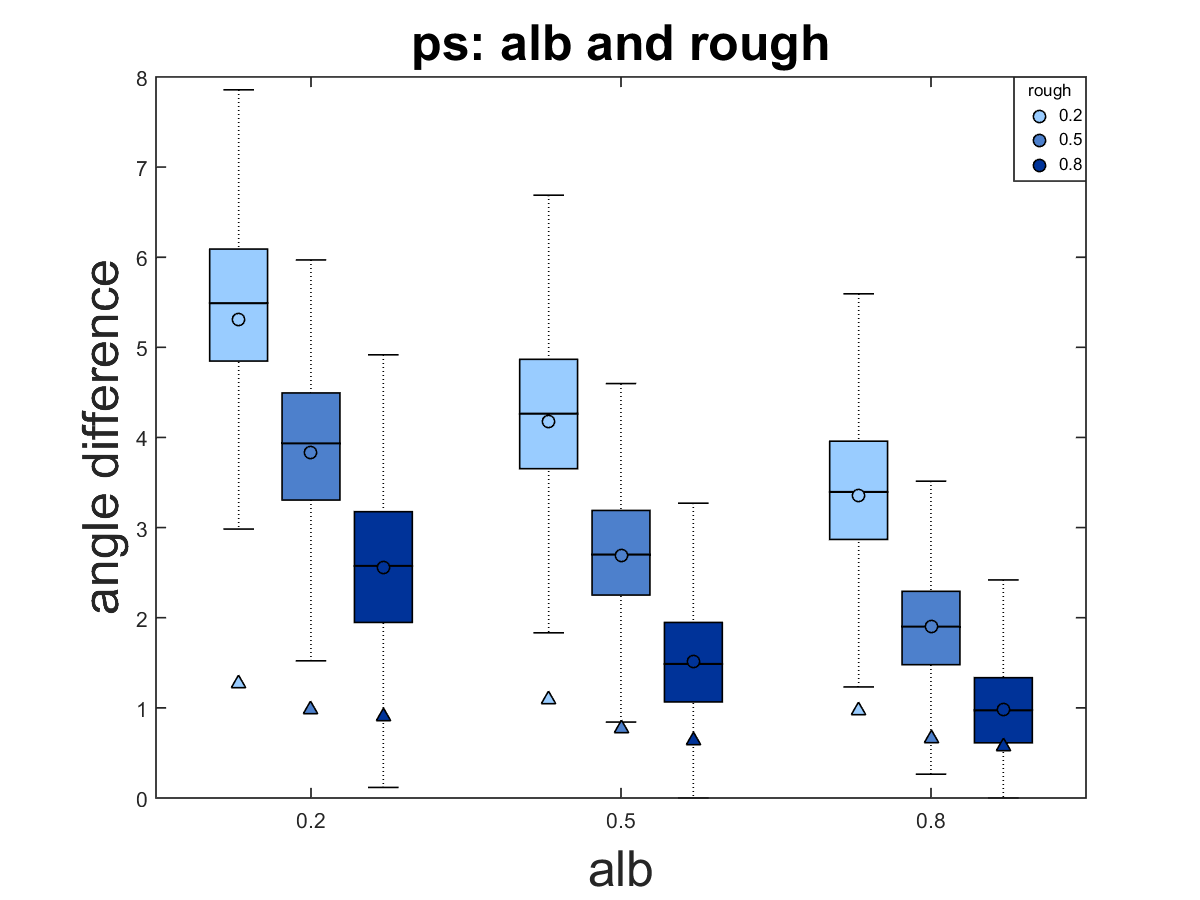
\includegraphics[width=0.3\textwidth]{mapping/depend_check/ps_alb_rough}&
\includegraphics[width=0.3\textwidth]{mapping/depend_check/ps_spec_rough}\\
(d) & (e) & (f)\\
\end{tabular}
\caption{Performance of Example-based PS under six pairwise conditions. For instance, (a) shows the performance under changing \textit{texture} and \textit{albedo} values. The property values are assigned based on the settings in Table~\ref{tab:ps_depend_check_params} (a).}
\label{fig:ps_depend_check}
\end{sidewaysfigure}

\subsubsection{Effective and Dependent Properties}
We investigate how each property affects the reconstruction in terms of the statistics of the angular difference.

\textbf{(a) Texture and Albedo} 
Texture has no effect on angular difference while albedo has a positive effect on normal estimation.

\textbf{(b) Texture and Specular} 
Texture has no effect on angular difference while specular has a negative effect on normal estimation since the difference of mean and median gets larger as the specular increases. This can be explained as follows: as the specular increases, only the specular regions exhibit erroneous normal estimation while the rest of the surface is reliably estimated, see Figure~\ref{fig:ps_tex_spec}. That is why the median value exhibits far less change while the mean value increases significantly as shown in Figure~\ref{fig:ps_depend_check} (b).
\begin{figure}[!htbp]
\centering
\begin{tabular}{c|ccc}
Image & Normal map & Height map & Angular error\\
\hline\\
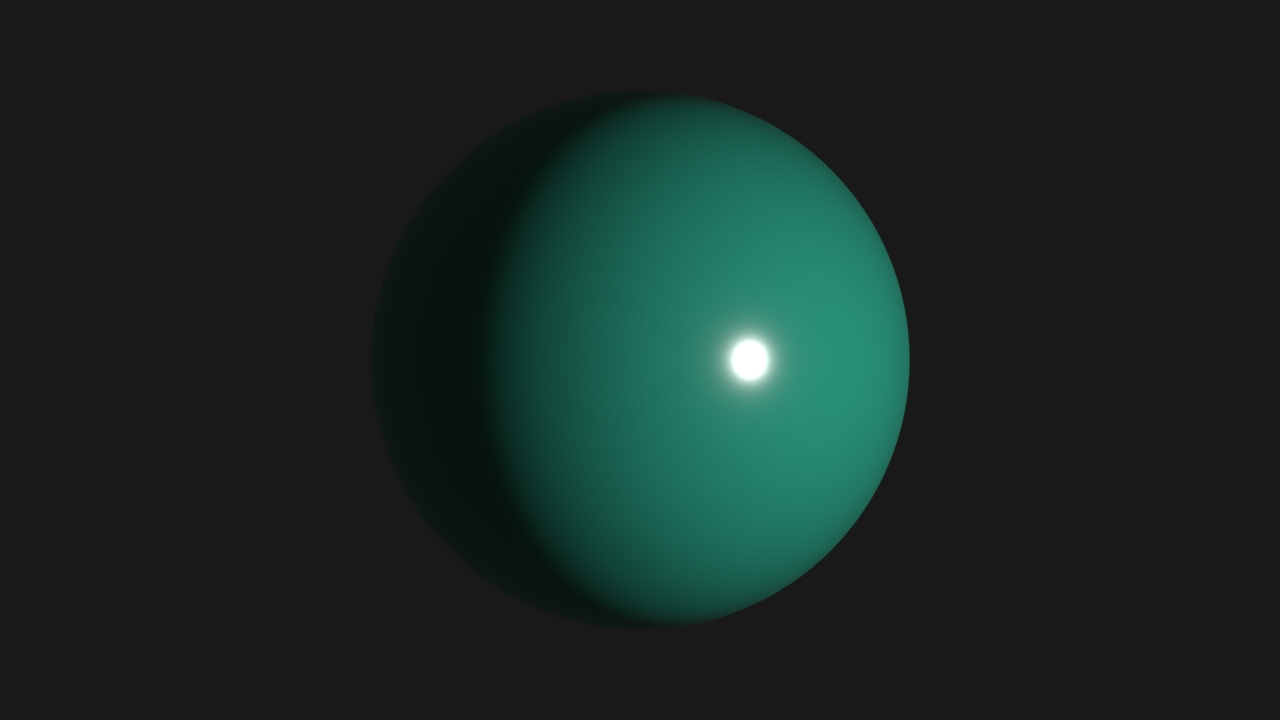
\includegraphics[width=0.33\textwidth]{mapping/ps_tex_spec/0502_0001}&
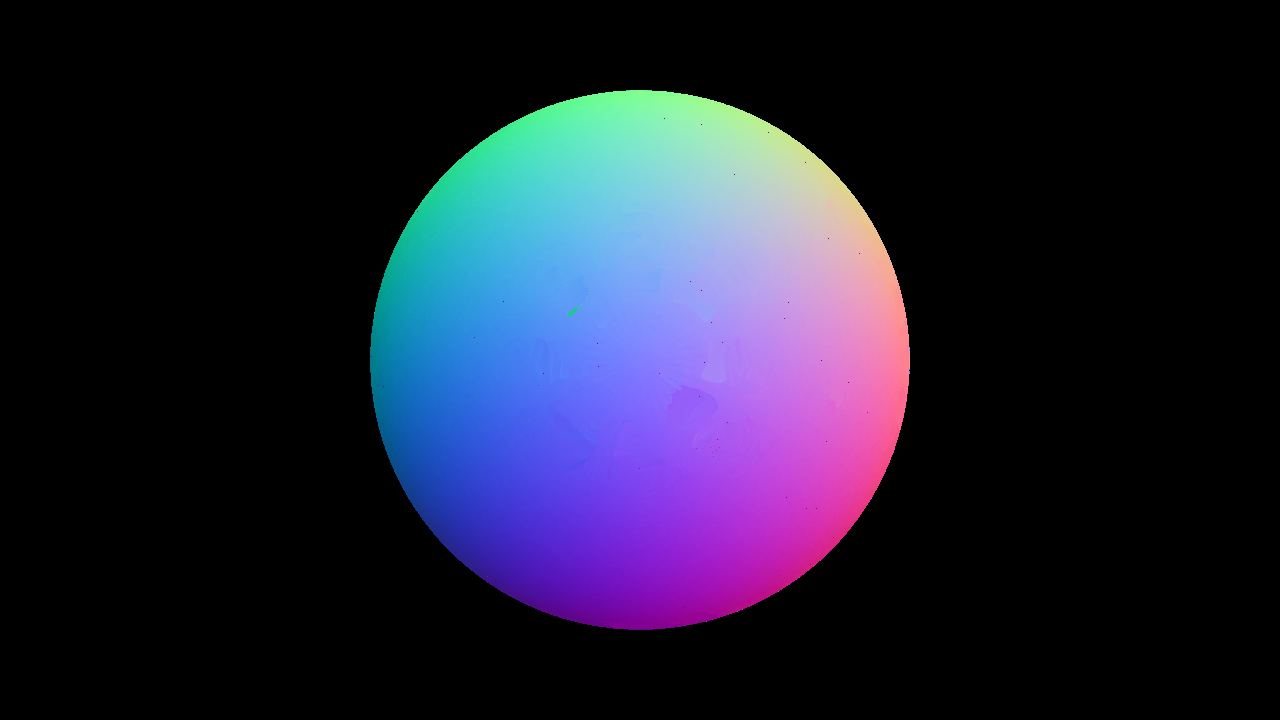
\includegraphics[width=0.33\textwidth]{mapping/ps_tex_spec/0502_normal}&
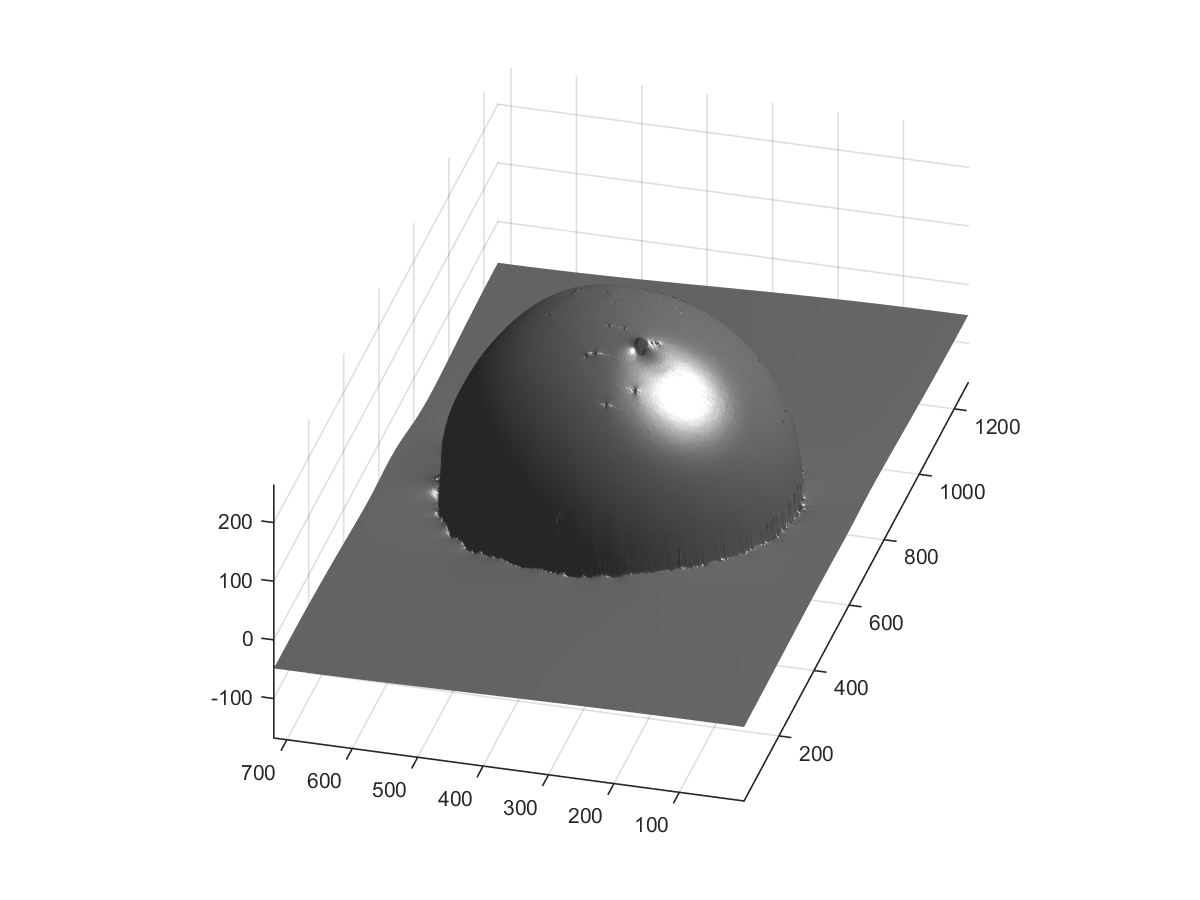
\includegraphics[width=0.25\textwidth]{mapping/ps_tex_spec/0502_dmap}&
\includegraphics[width=0.06\textwidth]{mapping/ps_tex_spec/0502_ang_error}\\
 & spec: 0.2 & \\
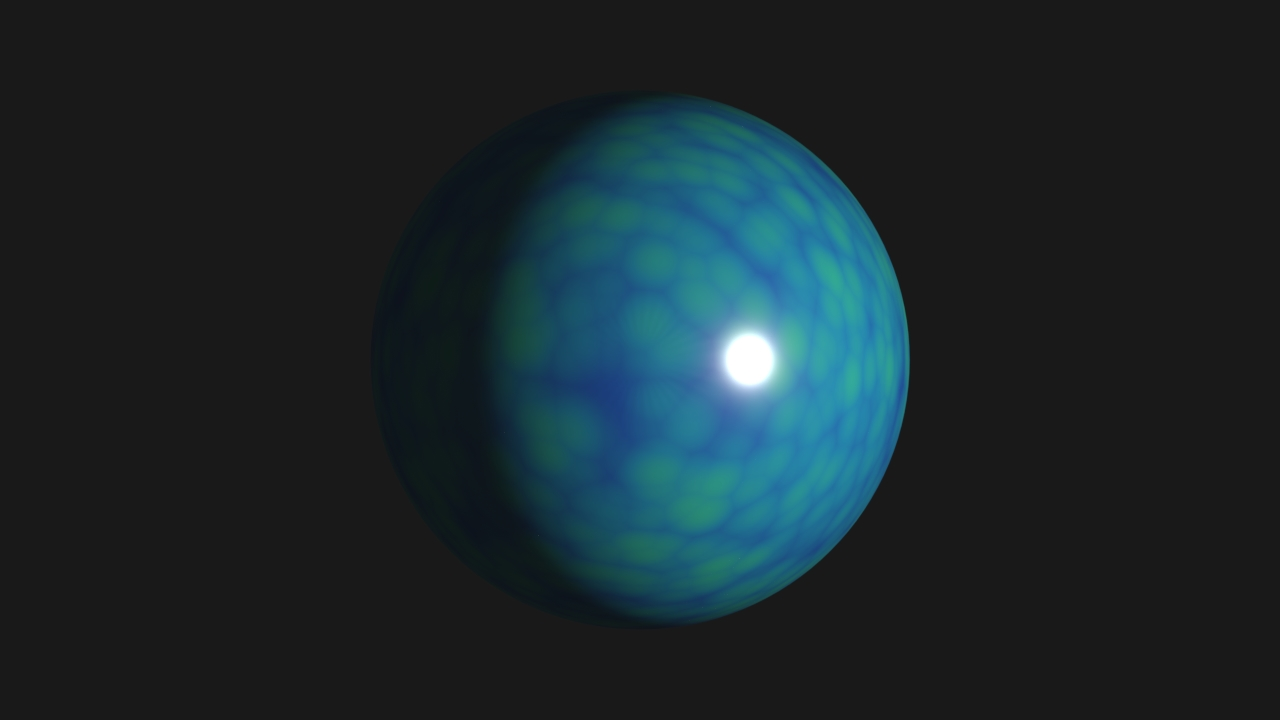
\includegraphics[width=0.33\textwidth]{mapping/ps_tex_spec/0505_0001}&
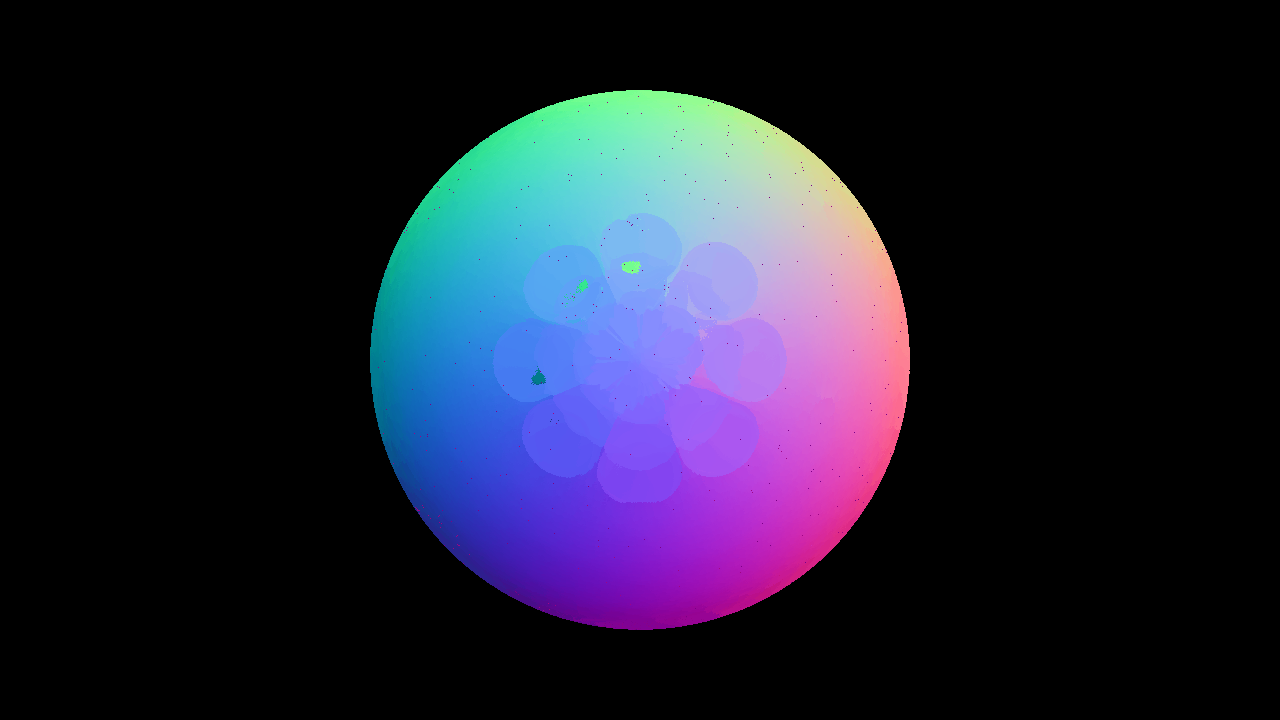
\includegraphics[width=0.33\textwidth]{mapping/ps_tex_spec/0505_normal}&
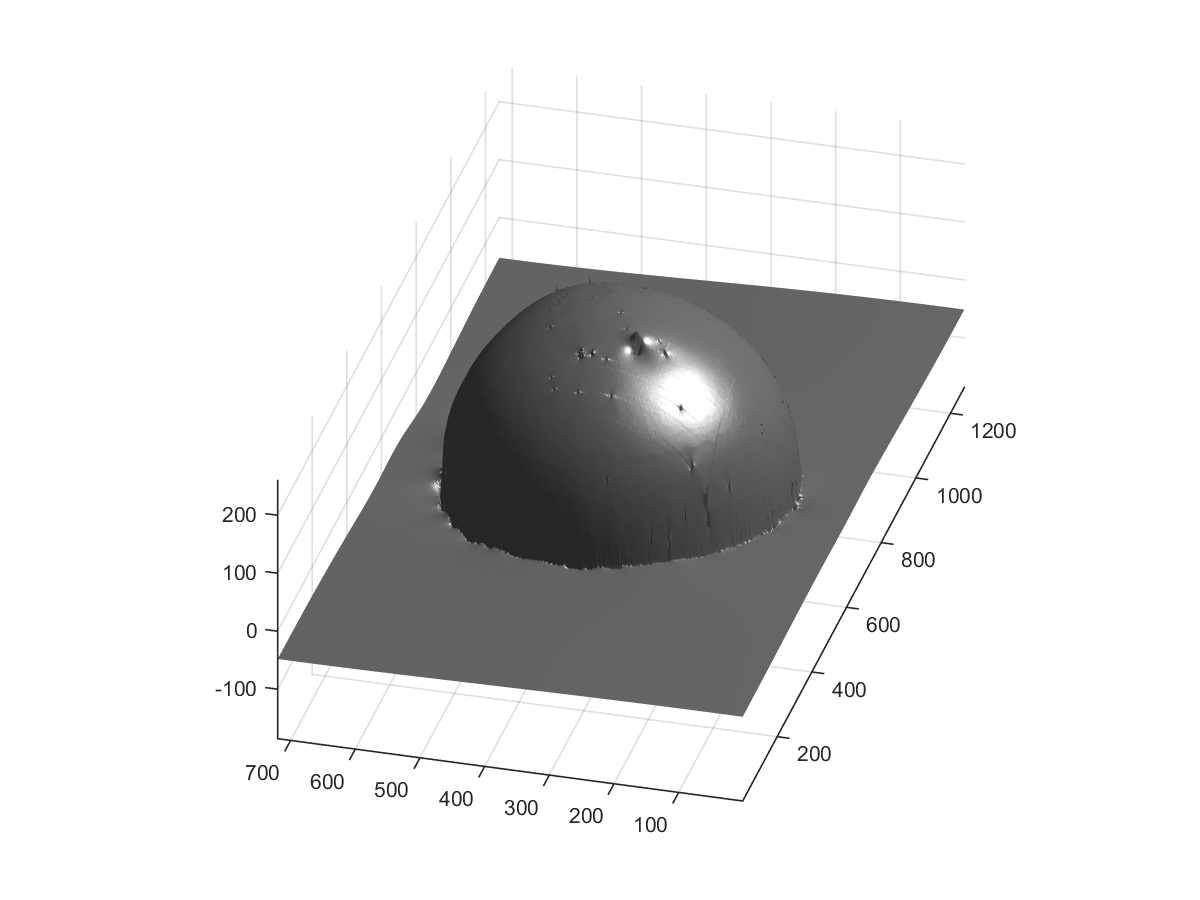
\includegraphics[width=0.25\textwidth]{mapping/ps_tex_spec/0505_dmap}&
\includegraphics[width=0.06\textwidth]{mapping/ps_tex_spec/0505_ang_error}\\
 & spec: 0.5 & \\
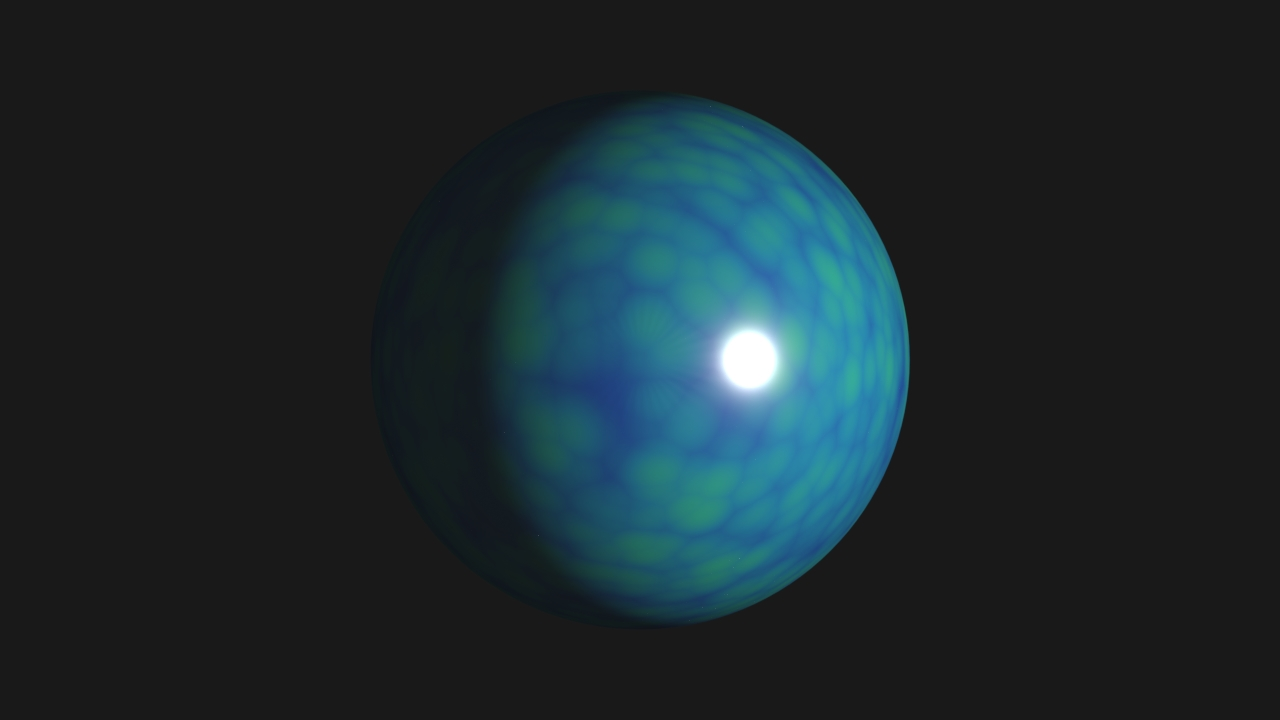
\includegraphics[width=0.33\textwidth]{mapping/ps_tex_spec/0508_0001}&
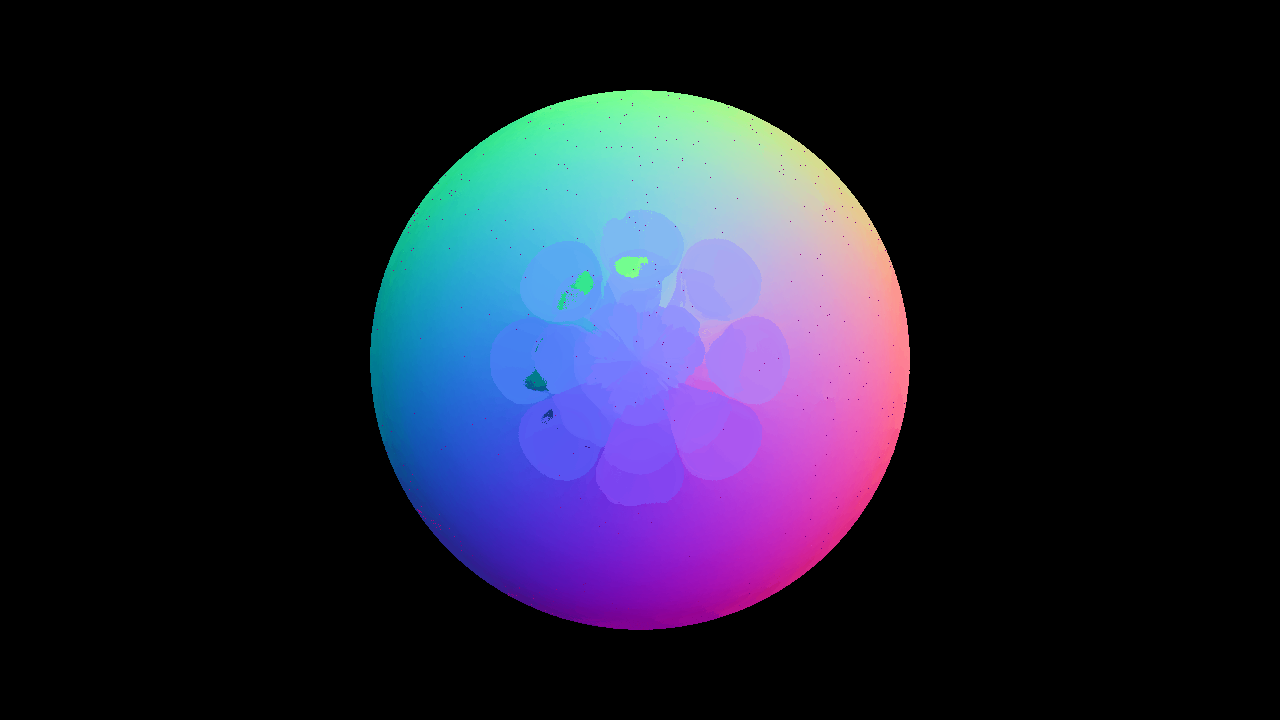
\includegraphics[width=0.33\textwidth]{mapping/ps_tex_spec/0508_normal}&
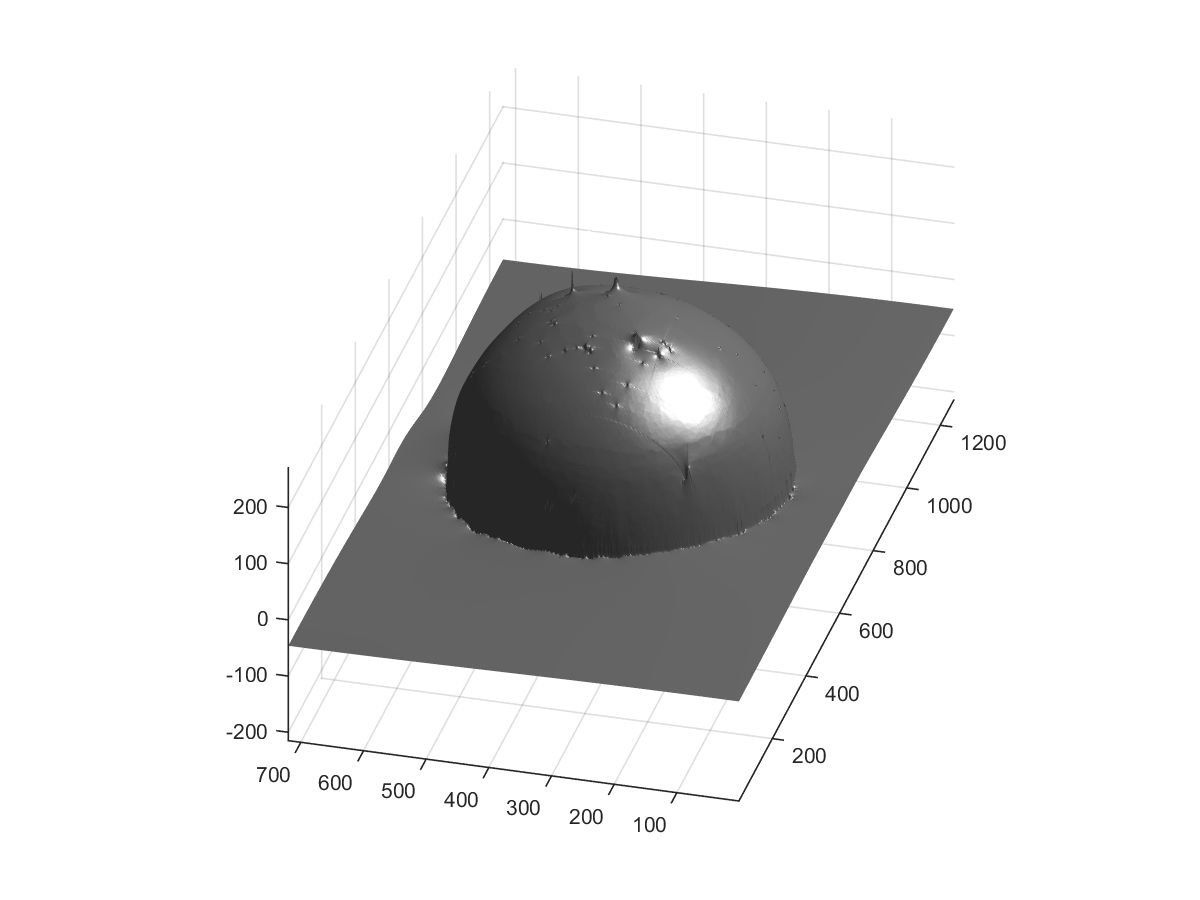
\includegraphics[width=0.25\textwidth]{mapping/ps_tex_spec/0508_dmap}&
\includegraphics[width=0.06\textwidth]{mapping/ps_tex_spec/0508_ang_error}\\
 & spec: 0.8 & \\
\end{tabular}
\caption{(a)-(c). The texture is set as 0.5. The estimated normal map and recovered surface becomes consistently worse as the specular level rises.}
\label{fig:ps_tex_spec}
\end{figure}

\textbf{(c) Texture and Roughness} 
Texture has no effect on angular difference while roughness has a positive effect on normal estimation.

\textbf{(d) Albedo and Specular} 
The albedo has a positive impact on normal estimation, see Figure~\ref{fig:ps_alb_spec} (a)-(c) whereas the specular a negative impact on normal estimation, see Figure~\ref{fig:ps_alb_spec} (d)-(f).
\begin{figure}[!htbp]
\centering
\begin{tabular}{c|ccc}
Image & Normal map & Height map & Angular error\\
\hline\\
% 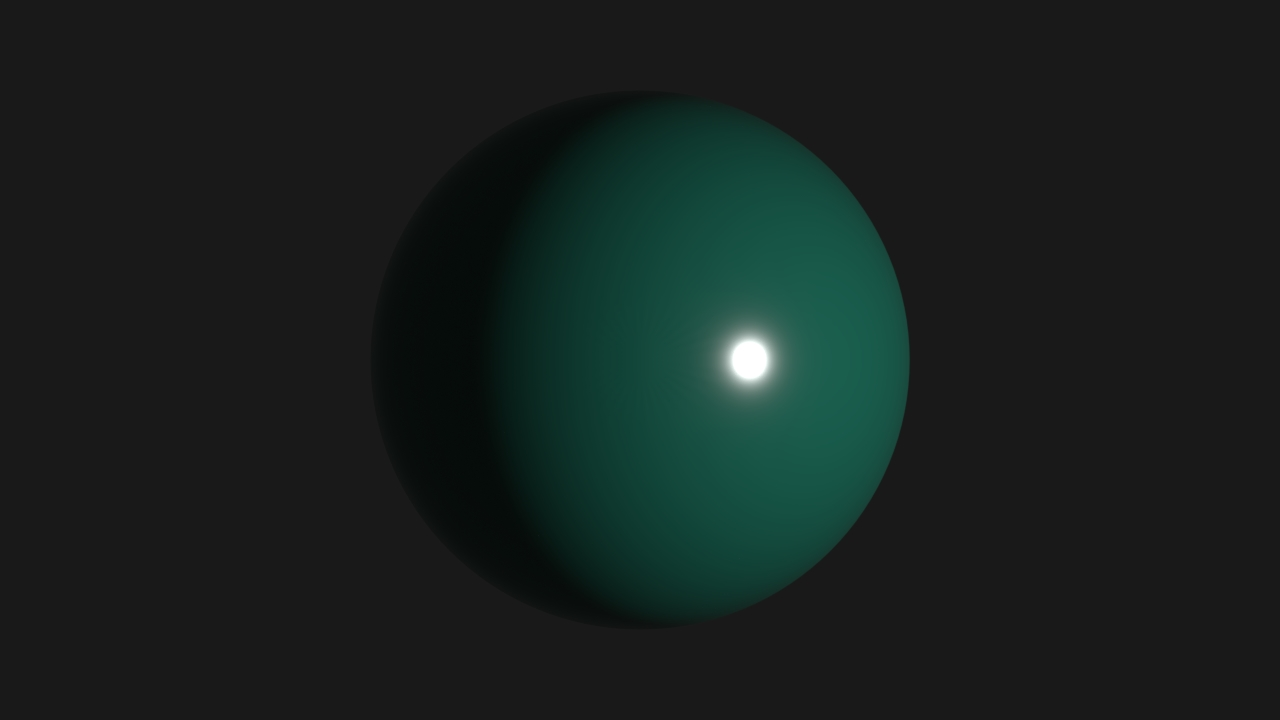
\includegraphics[width=0.33\textwidth]{mapping/ps_alb_spec/0202_0001}&
% 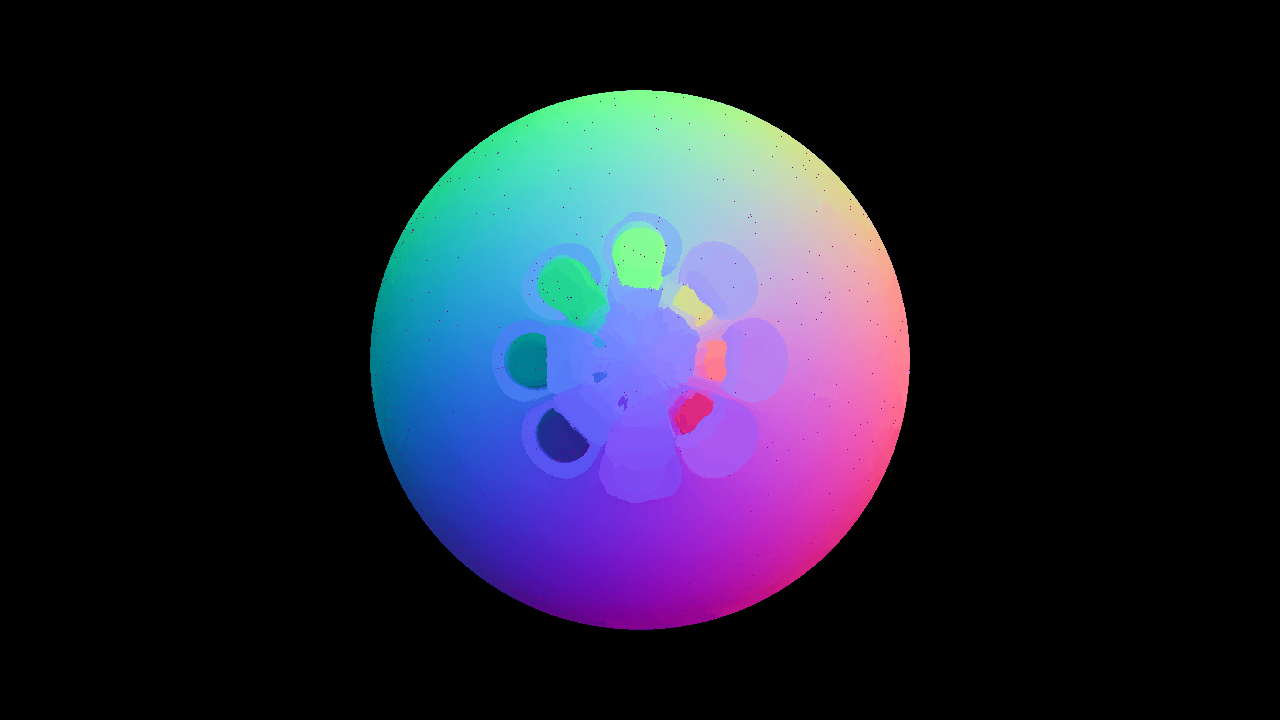
\includegraphics[width=0.33\textwidth]{mapping/ps_alb_spec/0202_normal}&
% 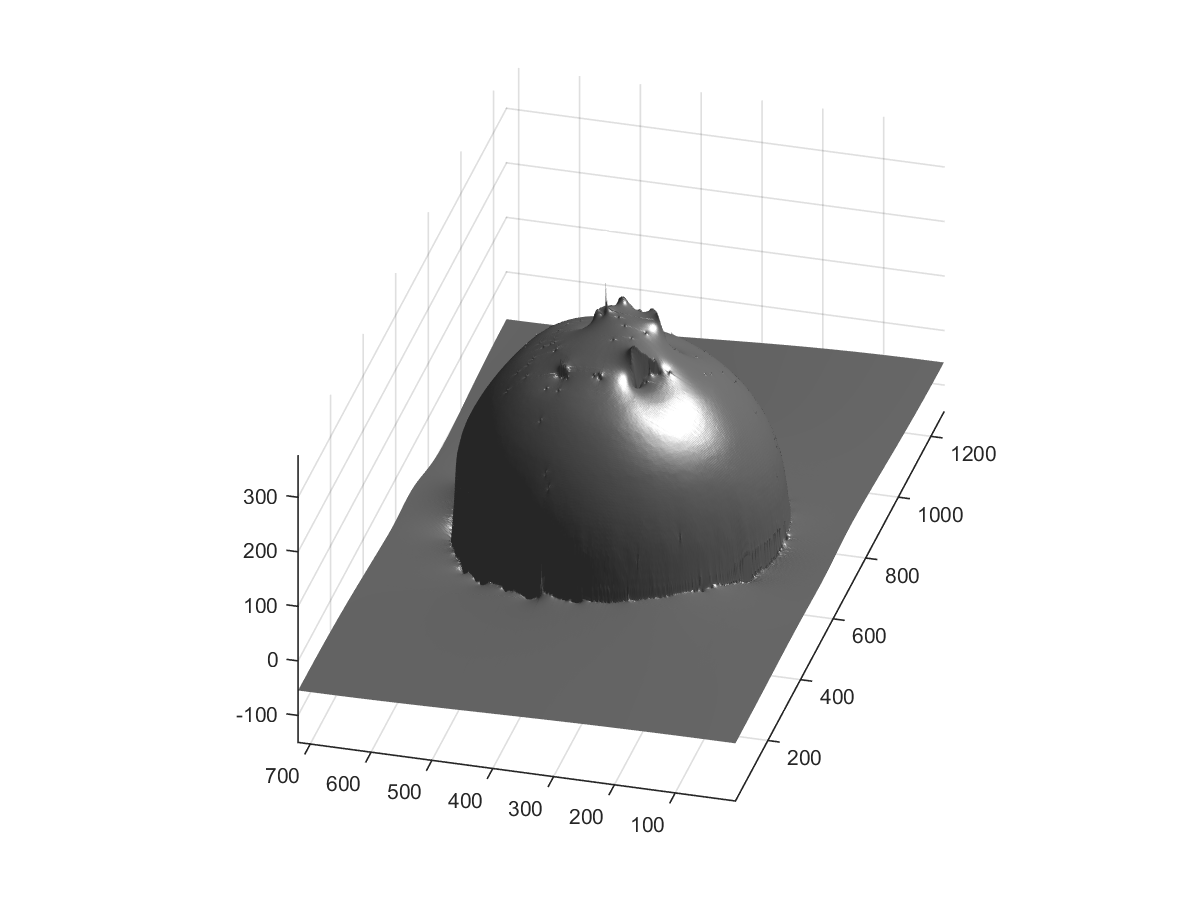
\includegraphics[width=0.25\textwidth]{mapping/ps_alb_spec/0202_dmap}&
% \includegraphics[width=0.06\textwidth]{mapping/ps_alb_spec/0202_ang_error}\\
%  & (a) albedo: 0.2, spec: 0.2 & \\
\includegraphics[width=0.33\textwidth]{mapping/ps_alb_spec/0802_0001}&
\includegraphics[width=0.33\textwidth]{mapping/ps_alb_spec/0802_normal}&
\includegraphics[width=0.25\textwidth]{mapping/ps_alb_spec/0802_dmap}&
\includegraphics[width=0.06\textwidth]{mapping/ps_alb_spec/0802_ang_error}\\
 & (a) albedo: 0.8, spec: 0.2 & \\
\includegraphics[width=0.33\textwidth]{mapping/ps_alb_spec/0502_0001}&
\includegraphics[width=0.33\textwidth]{mapping/ps_alb_spec/0502_normal}&
\includegraphics[width=0.25\textwidth]{mapping/ps_alb_spec/0502_dmap}&
\includegraphics[width=0.06\textwidth]{mapping/ps_alb_spec/0502_ang_error}\\
 & (b) albedo: 0.5, spec: 0.2 & \\
\includegraphics[width=0.33\textwidth]{mapping/ps_alb_spec/0202_0001}&
\includegraphics[width=0.33\textwidth]{mapping/ps_alb_spec/0202_normal}&
\includegraphics[width=0.25\textwidth]{mapping/ps_alb_spec/0202_dmap}&
\includegraphics[width=0.06\textwidth]{mapping/ps_alb_spec/0202_ang_error}\\
 & (c) albedo: 0.2, spec: 0.2 & \\
\includegraphics[width=0.33\textwidth]{mapping/ps_alb_spec/0205_0001}&
\includegraphics[width=0.33\textwidth]{mapping/ps_alb_spec/0205_normal}&
\includegraphics[width=0.25\textwidth]{mapping/ps_alb_spec/0205_dmap}&
\includegraphics[width=0.06\textwidth]{mapping/ps_alb_spec/0205_ang_error}\\
 & (d) albedo: 0.2, spec: 0.5 & \\
\includegraphics[width=0.33\textwidth]{mapping/ps_alb_spec/0208_0001}&
\includegraphics[width=0.33\textwidth]{mapping/ps_alb_spec/0208_normal}&
\includegraphics[width=0.25\textwidth]{mapping/ps_alb_spec/0208_dmap}&
\includegraphics[width=0.06\textwidth]{mapping/ps_alb_spec/0208_ang_error}\\
 & (e) albedo: 0.2, spec: 0.8 & \\
\end{tabular}
\caption{According to energy conservation, as the specular component increases, the diffuse component decreases. (a)-(c): the estimated normal map and recovered height map becomes consistently worse as the albedo decreases; (c)-(e): the estimated normal map and recovered height map becomes consistently worse as the specular increaess.}
\label{fig:ps_alb_spec}
\end{figure}

\textbf{(e) Albedo and Roughness} 
Both albedo and roughness have a positive effect on normal estimation.

\textbf{(f) Specular and Roughness} 
The specular has a negative impact on normal estimation. However, the roughness has a more complicated effect. We observed that the reconstruction becomes worse when roughness is 0.5, which is counter-intuitive at first sight. However, we argue that it's because the roughness is not strong enough to counteract the specular component, thus resulting in a smoothed and blurred specular lobe with larger area, thus leading to a worse reconstruction result. This effect is also demonstrated in the training stage, see Figure~\ref{fig:ps_spec_rough} for some visual examples.
\begin{figure}[h!]
\centering
\begin{tabular}{c|ccc}
  Image & Normal map & Height map & Angular error\\
  \hline\\
  \includegraphics[width=0.33\textwidth]{mapping/ps_spec_rough/0802_0001}&
  \includegraphics[width=0.33\textwidth]{mapping/ps_spec_rough/0802_normal}&
  \includegraphics[width=0.25\textwidth]{mapping/ps_spec_rough/0802_dmap}&
  \includegraphics[width=0.06\textwidth]{mapping/ps_spec_rough/0802_ang_error}\\
  & (a). rough: 0.2\\
  \includegraphics[width=0.33\textwidth]{mapping/ps_spec_rough/0805_0001}&
  \includegraphics[width=0.33\textwidth]{mapping/ps_spec_rough/0805_normal}&
  \includegraphics[width=0.25\textwidth]{mapping/ps_spec_rough/0805_dmap}&
  \includegraphics[width=0.06\textwidth]{mapping/ps_spec_rough/0805_ang_error}\\
  & (b). rough: 0.5\\
  \includegraphics[width=0.33\textwidth]{mapping/ps_spec_rough/0808_0001}&
  \includegraphics[width=0.33\textwidth]{mapping/ps_spec_rough/0808_normal}&
  \includegraphics[width=0.25\textwidth]{mapping/ps_spec_rough/0808_dmap}&
  \includegraphics[width=0.06\textwidth]{mapping/ps_spec_rough/0808_ang_error}\\
  & (c). rough: 0.8\\
\end{tabular}
\caption{The `peculiar' effect of roughness on PS. Albedo is set as 0.8, and specular is set as 0.8. (b) demonstrate that a medium level roughness would lead to worse normal estimation since it blurs the specular lobe.}
\label{fig:ps_spec_rough}
\end{figure}

\subsubsection{Summary} 
The properties that have an effect on the EPS are: albedo, specular, and roughness, as shown in Table~\ref{tab:ps_depend_prop}. Therefore, we will only consider these three properties for all the forthcoming discussion of EPS.
\begin{table}[!htbp]
  \centering
  \begin{tabular}{l*{5}{c}}
  \hline
  \textbf{Metric} & Texture & Albedo & Specular & Roughness\\
  \hline
  Angle difference & \ding{55} & \checkmark & \checkmark & \checkmark\\
  \hline
  \end{tabular}
  \caption{The \textit{effective problem domain} of EPS in terms of the \textit{angular difference}.}
  \label{tab:ps_depend_prop}
\end{table}

\subsection{EPD of GSL}
We evaluate the performance of Gray-code SL in terms of accuracy and completeness under varied combination of properties, the settings of the properties are listed in Table~\ref{tab:sl_depend_check_params}.
\begin{table}[!htbp]
  \centering
  \begin{tabular}{l*{4}{c}}
  \hline
  \textbf{Property} & Texture & Albedo & Specular & Roughness\\
  \hline
  \textbf{(a)} & [0.2, 0.8] & [0.2, 0.8] & 0.0 & 0.0\\
  \textbf{(b)} & [0.2, 0.8] & 0.8 & [0.2, 0.8] & 0.0\\
  \textbf{(c)} & [0.2, 0.8] & 0.8 & 0.0 & [0.2, 0.8]\\
  \textbf{(d)} & 0.0 & [0.2, 0.8] & [0.2, 0.8] & 0.0\\
  \textbf{(e)} & 0.0 & [0.2, 0.8] & 0.0 & [0.2, 0.8]\\
  \textbf{(f)} & 0.0 & 0.8 & [0.2, 0.8] & [0.2, 0.8]\\
  \hline
  \end{tabular}
  \caption{Problem conditions for establishing the \textit{effective problem domain} of GSL.}
  \label{tab:sl_depend_check_params}
\end{table}

\begin{sidewaysfigure}[!htbp]
\begin{tabular}{ccc}
\includegraphics[width=0.3\textwidth]{mapping/depend_check/sl_tex_alb}&
\includegraphics[width=0.3\textwidth]{mapping/depend_check/sl_tex_spec}&
\includegraphics[width=0.3\textwidth]{mapping/depend_check/sl_tex_rough}\\
(a) & (b) & (c)\\
\includegraphics[width=0.3\textwidth]{mapping/depend_check/sl_alb_spec}&
\includegraphics[width=0.3\textwidth]{mapping/depend_check/sl_alb_rough}&
\includegraphics[width=0.3\textwidth]{mapping/depend_check/sl_spec_rough}\\
(d) & (e) & (f)\\
\end{tabular}
\caption{Performance of Gray-encoded SL under six pairwise conditions. For instance, (a) shows the performance under changing \textit{texture} and \textit{albedo} values. The property values are assigned based on settings in Table~\ref{tab:sl_depend_check_params} (a).}
\label{fig:sl_depend_check}
\end{sidewaysfigure}

\subsubsection{Effective and Dependent Properties}
We investigate how each property affects the reconstruction in terms of accuracy and completeness. A depth check step is performed to remove erroneous depth, thus the accuracy remain almost constant across all cases.

\textbf{(a) Texture and Albedo} 
Texture has no significant effect whereas albedo has a positive effect on compleness. Both properties have no significant effect on accuracy.

\textbf{(b) Texture and Specular} 
Texture has no significant effect whereas specular has a negative effect on compleness. Both properties have no significant effect on accuracy.

\textbf{(c) Texture and Roughness} 
Texture has no significant effect whereas roughness has a slightly positive effect on compleness. Both properties have no significant effect on accuracy.

\textbf{(d) Albedo and Specular} 
Albedo has a positive effect, see Figure~\ref{fig:sl_alb_spec} (a)-(c) whereas specular a negative effect on completeness, see Figure~\ref{fig:sl_alb_spec} (d)-(f). Th effect of specular becomes less substantial as the albedo increases, see Figure~\ref{fig:sl_depend_check} (d). Thus we conclude that the effect of specular is most significant when the albedo is low. Neither property has a significant effect on accuracy.
\begin{figure}[!htbp]
\centering
\begin{tabular}{ccc}
\includegraphics[width=0.33\textwidth]{mapping/sl_alb_spec/sl_00020202}&
\includegraphics[width=0.33\textwidth]{mapping/sl_alb_spec/sl_00050202}&
\includegraphics[width=0.33\textwidth]{mapping/sl_alb_spec/sl_00080202}\\
(a) albedo: 0.2 & (b) albedo: 0.5 & (c) albedo: 0.8\\
\includegraphics[width=0.33\textwidth]{mapping/sl_alb_spec/sl_00020202}&
\includegraphics[width=0.33\textwidth]{mapping/sl_alb_spec/sl_00020502}&
\includegraphics[width=0.33\textwidth]{mapping/sl_alb_spec/sl_00020802}\\
(d) specular: 0.2 & (e) specular: 0.5 & (f) specular: 0.8\\
\end{tabular}
\caption{(a)-(c): the specular is set as 0.2, albedo has a positive effect on completeness; (d)-(e): the albedo is set as 0.2, specular has a negative effect on completeness.}
\label{fig:sl_alb_spec}
\end{figure}

\textbf{(e) Albedo and Roughness} 
Albedo has a positive effect whereas roughness has a slightly positive effect on compleness. Both properties have no significant effect on accuracy.

\textbf{(f) Specular and Roughness} 
Specular has a negative effect, see Figure~\ref{fig:sl_spec_rough} (a)-(c) whereas roughness has a positive effect on completeness, see Figure~\ref{fig:sl_spec_rough} (d)-(f). Neither property has a significant effect on accuracy.
\begin{figure}[!htbp]
\centering
\begin{tabular}{ccc}
\includegraphics[width=0.33\textwidth]{mapping/sl_spec_rough/sl_00050202}&
\includegraphics[width=0.33\textwidth]{mapping/sl_spec_rough/sl_00050502}&
\includegraphics[width=0.33\textwidth]{mapping/sl_spec_rough/sl_00050802}\\
(a) specular: 0.2 & (b) specular: 0.5 & (c) specular: 0.8\\
\includegraphics[width=0.33\textwidth]{mapping/sl_spec_rough/sl_00050802}&
\includegraphics[width=0.33\textwidth]{mapping/sl_spec_rough/sl_00050805}&
\includegraphics[width=0.33\textwidth]{mapping/sl_spec_rough/sl_00050808}\\
(d) roughness: 0.2 & (e) roughness: 0.5 & (f) roughness: 0.8\\
\end{tabular}
\caption{(a)-(c): the roughness is set as 0.2, specular has a negative effect on completeness; (d)-(e): the specular is set as 0.8, roughness has a positive effect on competeness.}
\label{fig:sl_spec_rough}
\end{figure}

\subsubsection{Summary}
The properties that have an effect on the GSL are: texture, albedo, specular, as shown in Table~\ref{tab:sl_depend_prop}. Therefore, we will only consider these three properties for all forthcoming discussion of GSL.
\begin{table}[!htbp]
  \centering
  \begin{tabular}{l*{4}{c}}
  \hline
  \textbf{Metric} & Texture & Albedo & Specular & Roughness\\
  \hline
  Accuracy & \ding{55} & \ding{55} & \ding{55} & \ding{55}\\
  Completeness & \ding{55} & \checkmark & \checkmark & \checkmark\\
  \hline
  \end{tabular}
  \caption{The \textit{effective problem domain} of GSL in terms of accuracy and completeness.}
  \label{tab:sl_depend_prop}
\end{table}

\section{Mapping Construction}
We generate another synthetic dataset using only the effective and dependent properties and all their combinations. Since there are three effective properties for each selected method, there are in total $L^3$ different combinations of property values for each technique, where $L$ is the number of discrete values for each property, which is set as 3 representing the discrete values of $0.2, 0.5, 0.8$. We present the results as follows: the $27(3^3)$ results are divided into three plots. Each plot illustrates the results of one fixed property $P_1$, and two changing properties $P_2$ and $P_3$. To have a better understanding of the pairwise relation between any two properties, each effective property would be chosen as $P_1$ once. Therefore, we end up with three groups of graphs with each consisting of three plots.

\subsection{Mapping of PMVS}
The performances of PMVS under different combinations of property values are shown in Figure~\ref{fig:mvs_training}, along with the performance of the baseline method. The conditions under which PMVS works well are listed in Table~\ref{tab:mvs_training_result}. We make the following observations from the training results:
\begin{figure}[!htbp]
\begin{tabular}{ccc}
\includegraphics[width=0.33\textwidth]{mapping/training/mvs_train_spec_02}&
\includegraphics[width=0.33\textwidth]{mapping/training/mvs_train_spec_05}&
\includegraphics[width=0.33\textwidth]{mapping/training/mvs_train_spec_08}\\
(a) & (b) & (c)\\
\includegraphics[width=0.33\textwidth]{mapping/training/mvs_train_tex_02}&
\includegraphics[width=0.33\textwidth]{mapping/training/mvs_train_tex_05}&
\includegraphics[width=0.33\textwidth]{mapping/training/mvs_train_tex_08}\\
(d) & (e) & (f)\\
\includegraphics[width=0.33\textwidth]{mapping/training/mvs_train_alb_02}&
\includegraphics[width=0.33\textwidth]{mapping/training/mvs_train_alb_05}&
\includegraphics[width=0.33\textwidth]{mapping/training/mvs_train_alb_08}\\
(g) & (h) & (i)\\
\end{tabular}
\caption{Performance of PMVS under varied conditions of changing property values. The baseline method serves as the guidelines to determine the performance of PMVS.}
\label{fig:mvs_training}
\end{figure}

\noindent\textbf{(a)-(c) Texture}: as the texture level increases, the completeness increases consistently, and accuracy also improves for medium/high albedo and low-medium specular surfaces.

\noindent\textbf{(d)-(f) Albedo}: for medium/high textured surfaces, albedo can effectively counteract the effect of specular, \ie improve both the accuracy and completenss of the reconstruction, see the red and green lines in Figure~\ref{fig:mvs_training} (d)-(f). As for low textured surface, the effect of albedo is less significant, see the blue line in Figure~\ref{fig:mvs_training} (d)-(f).

\noindent\textbf{(g)-(i) Specular}: the effect of specular is closely related to albedo: surface with higher albedo is able to endure higher specular component, see the performance difference between the red (alb = 0.5) and green (alb = 0.8) line in Figure~\ref{fig:mvs_train} (g) - (i). For low/medium textured surface, Specular has a consistently negative impact for low/medium textured surface whereas the effect is almost neutralized for highly textured surfaces. This aligns with previous observation illustrated in Figure~\ref{fig:mvs_spec}.

We could derive the problem conditions that PMVS could reliably work on from the training results. Those conditions are listed in Table~\ref{tab:mvs_training_result}.
\begin{table}[!htbp]
  \centering
  \begin{tabular}{l*{4}{c}}
  \hline
  \textbf{Metric} & Texture & Albedo & Specular & Roughness\\
  \hline
  Accuracy & 0.5 & 0.5 & 0.2 & -\\
           & 0.5 & 0.8 & 0.2 & -\\
           & 0.8 & 0.2 & 0.2 & -\\
           & 0.8 & 0.5 & 0.2 & -\\
           & 0.8 & 0.8 & 0.2 & -\\
           & 0.8 & 0.5 & 0.5 & -\\
           & 0.8 & 0.8 & 0.5 & -\\
           & 0.8 & 0.5 & 0.8 & -\\
           & 0.8 & 0.8 & 0.8 & -\\
  \hline
  Completeness & 0.5 & 0.5 & 0.2 & -\\
               & 0.5 & 0.8 & 0.2 & -\\
               & 0.5 & 0.8 & 0.5 & -\\
               & 0.8 & 0.2 & 0.2 & -\\
               & 0.8 & 0.5 & 0.2 & -\\
               & 0.8 & 0.8 & 0.2 & -\\
               & 0.8 & 0.5 & 0.5 & -\\
               & 0.8 & 0.8 & 0.5 & -\\
               & 0.8 & 0.5 & 0.8 & -\\
               & 0.8 & 0.8 & 0.8 & -\\
  \hline
  \end{tabular}
  \caption{The condition matrix of PMVS in terms of the two metrics \textit{accuracy} and \textit{completeness}.}
  \label{tab:mvs_training_result}
\end{table}

\subsection{Mapping of EPS}
The performances of example-based PS under difference combinations of properties are shown in Figure~\ref{fig:ps_training}, along with the result of te baseline method. The conditions under which example-based PS works well are listed in Table~\ref{tab:ps_training_result}. We make the following observations from the training results:
\begin{figure}[!htbp]
\begin{tabular}{cccc}
\includegraphics[width=0.3\textwidth]{mapping/training/ps_rough_02}&
\includegraphics[width=0.3\textwidth]{mapping/training/ps_rough_05}&
\includegraphics[width=0.3\textwidth]{mapping/training/ps_rough_08}&
\includegraphics[width=0.087\textwidth]{mapping/training/ps_baseline}\\
(a) & (b) & (c)\\
\includegraphics[width=0.3\textwidth]{mapping/training/ps_alb_02}&
\includegraphics[width=0.3\textwidth]{mapping/training/ps_alb_05}&
\includegraphics[width=0.3\textwidth]{mapping/training/ps_alb_08}&
\includegraphics[width=0.087\textwidth]{mapping/training/ps_baseline}\\
(d) & (e) & (f)\\
\includegraphics[width=0.3\textwidth]{mapping/training/ps_spec_02}&
\includegraphics[width=0.3\textwidth]{mapping/training/ps_spec_05}&
\includegraphics[width=0.3\textwidth]{mapping/training/ps_spec_08}&
\includegraphics[width=0.087\textwidth]{mapping/training/ps_baseline}\\
(g) & (h) & (i)\\
\end{tabular}
\caption{Performance of EPS under varied conditions of changing property values. Varied statistical measures of angular error are compared to the baseline method to determine the performance of EPS.}
\label{fig:ps_training}
\end{figure}

\noindent\textbf{(a)-(c) Albedo}: albedo has a consistently positive effect on the reconstruction.

\noindent\textbf{(d)-(f) Specular}: specular has a consistently negative impact on the normal estimation, which is manifested by the increasing variation represented by interquartile range and standard deviation.

\noindent\textbf{(g)-(i) Roughness}: roughness has a more complicated effect on reconstruction as illustrated in Figure~\ref{fig:ps_spec_rough}, \ie medium roughness would blur the specular area, and lead to worse normal estimation and shape recovery.

We could derive the problem conditions that EPS could reliably work on from the training results. Those conditions are in Table~\ref{tab:ps_training_result}.
\begin{table}[!htbp]
  \centering
  \begin{tabular}{l*{4}{c}}
  \hline
  \textbf{Metric} & Texture & Albedo & Specular & Roughness\\
  \hline
  Angle difference & - & 0.2 & 0.2 & 0.8\\
                   & - & 0.2 & 0.5 & 0.8\\
                   & - & 0.2 & 0.8 & 0.8\\
                   & - & 0.5 & 0.2 & 0.8\\
                   & - & 0.5 & 0.5 & 0.8\\
                   & - & 0.5 & 0.8 & 0.8\\
                   & - & 0.8 & 0.2 & 0.2\\ % can be removed
                   & - & 0.8 & 0.2 & 0.8\\
                   & - & 0.8 & 0.5 & 0.2\\
                   & - & 0.8 & 0.5 & 0.8\\
                   & - & 0.8 & 0.8 & 0.2\\ % can be removed
                   & - & 0.8 & 0.8 & 0.8\\
  \hline
  \end{tabular}
  \caption{The condition matrix of example-based PS in terms of the metric \textit{angular error}.}
  \label{tab:ps_training_result}
\end{table}

\subsection{Mapping of GSL}
The performances of Gray-code SL under different combinations of property values are shown in Figure~\ref{fig:sl_training}, along with the result of the baseline method. Only a portion of the scene is visible since there is only one camera, and the percent of visible surface varies from object to object. This value can be approximated by the completeness value obtained under the optimal reconstruction condition. In this case, we claim that the a completeness of $80\%$ of that of the baseline is acceptable. The conditions under which GSL works well are listed in Table~\ref{tab:sl_training_result}. We make the following observations:
\begin{figure}[!htbp]
\begin{tabular}{ccc}
\includegraphics[width=0.33\textwidth]{mapping/training/sl_train_rough_02}&
\includegraphics[width=0.33\textwidth]{mapping/training/sl_train_rough_05}&
\includegraphics[width=0.33\textwidth]{mapping/training/sl_train_rough_08}\\
(a) & (b) & (c)\\
\includegraphics[width=0.33\textwidth]{mapping/training/sl_train_alb_02}&
\includegraphics[width=0.33\textwidth]{mapping/training/sl_train_alb_05}&
\includegraphics[width=0.33\textwidth]{mapping/training/sl_train_alb_08}\\
(d) & (e) & (f)\\
\includegraphics[width=0.33\textwidth]{mapping/training/sl_train_spec_02}&
\includegraphics[width=0.33\textwidth]{mapping/training/sl_train_spec_05}&
\includegraphics[width=0.33\textwidth]{mapping/training/sl_train_spec_08}\\
(g) & (h) & (i)\\
\end{tabular}
\caption{Performance of GSL under varied conditions of changing property values. The baseline method serves as the guidelines to determine the performance of GSL.}
\label{fig:sl_training}
\end{figure}

\noindent\textbf{(a)-(i)}: the accuracy remains almost fixed, thus irrelevant to all properties;

\noindent\textbf{(a)-(c) Albedo}: albedo has a consistently positive effect on the completeness of the reconstruction.

\noindent\textbf{(d)-(f) Specular}: specular has a negative effect on completeness as shown in Figure~\ref{fig:sl_alb_spec} (d)-(f). However, we did notice in some case, the completeness of the reconstruction improves as the specular level increases. There are two contributing factors to completeness: 1). specular would decrease the completeness since the pattern can no longer be decoded in the glossy area, thus causing incomplete reconstruction; 2). large roughness would spread the specular lobe into a larger area, leading to a brighter surface, thus increase the completeness of the reconstruction. These two contradicting factors would together determine the completeness of the reconstruction. Thus if the first factor is more substantial, the completeness would decrease whereas if the second one is more significant, the completeness would increase.

\noindent\textbf{(g)-(i) Roughness}: roughness has similar effect as that we found on EPS, \ie medium roughness would blur the specular lobe to a larger area thus causing larger holes in the reconstruction, see Figure~\ref{fig:ps_spec_rough} (d)-(f). Large roughness would effectively counteract the effect of specular, thus improve the completeness of the reconstruction.

% However, we realize that the metric completeness doesn't always faithfully reflect the true quality of the reconstruction. Let's consider the following two cases: 1). with low albedo, high specular, 2). low albedo, median specular. We can see from the quantitative results that case 1 has higher completeness. However, case 2 has better reconstruction. The reason is that high specular would increase the lightness of the surface, and high lightness would lead to more reliably reconstructed points. Therefore, even though high specular leads to hole, these two factors eventually cancels out. Therefore, when deriving the mapping and comparing the results of SL. We should consider both the qualitative and quantitative results. 
We could derive the problem conditions under which GSL could reliably work by considering both the quantitative and qualitative results. Those conditions are listed in Table~\ref{tab:sl_training_result}.
\begin{table}[!htbp]
  \centering
  \begin{tabular}{l*{4}{c}}
  \hline
  \textbf{Metric} & Texture & Albedo & Specular & Roughness\\
  \hline
  Accuracy     & - & - & - & -\\
  \hline
  Completeness & - & 0.8 & 0.2 & 0.2\\
               & - & 0.8 & 0.5 & 0.2\\
               & - & 0.8 & 0.8 & 0.2\\
               & - & 0.8 & 0.2 & 0.8\\
               & - & 0.8 & 0.5 & 0.8\\
               & - & 0.8 & 0.8 & 0.8\\
  \hline
  \end{tabular}
  \caption{The condition matrix of Gray-code SL in terms of the two metrics \textit{accuracy} and \textit{completeness}.}
  \label{tab:sl_training_result}
\end{table}

\section{Summary}
The development of the mapping is an on-going process. For instance, we can include more quantitative metrics such as colour accuracy, `ghost reconstruction', etc. In order to make the mapping applicable to objects with more complex shapes, we need to consider more sophisticated geometric properties besides roughness, such as concavity, depth-discontinuity, occlusion, etc. Furthermore, the incorporation of more algorithms to another way to make sure that the problem space is well covered.


% \begin{table}[!htbp]
%   \centering
%   \begin{tabular}{*{7}{c}}
%   \hline
%   \multirow{2}{*}{Texture} & \multirow{2}{*}{Albedo} & \multirow{2}{*}{Specular} & \multirow{2}{*}{Roughness} & \multicolumn{3}{c}{Metrics}\\
%   & & & & Accuracy & Completeness & Ang Diff\\
%   0.8 & 0.2 & 0.2 & 0.2 & PMVS & PMVS & -\\
%   0.8 & 0.2 & 0.2 & 0.5 & PMVS & PMVS & -\\
%   0.8 & 0.2 & 0.2 & 0.8 & PMVS & PMVS & EPS\\
%   0.8 & 0.2 & 0.5 & 0.2 & PMVS & PMVS & -\\
%   0.8 & 0.2 & 0.5 & 0.5 & PMVS & PMVS & -\\
%   0.8 & 0.2 & 0.5 & 0.8 & PMVS, GSL & PMVS, GSL & EPS\\
%   0.8 & 0.2 & 0.8 & 0.2 & PMVS & PMVS & -\\
%   0.8 & 0.2 & 0.8 & 0.5 & PMVS & PMVS & -\\
%   0.8 & 0.2 & 0.8 & 0.8 & PMVS, GSL & PMVS, GSL & EPS\\
%   0.8 & 0.5 & 0.5 & 0.2 & PMVS & PMVS & -\\
%   0.8 & 0.5 & 0.5 & 0.5 & PMVS & PMVS & -\\
%   0.8 & 0.5 & 0.5 & 0.8 & PMVS, GSL & PMVS, GSL & EPS\\
%   0.8 & 0.5 & 0.8 & 0.2 & PMVS & PMVS & -\\
%   0.8 & 0.5 & 0.8 & 0.5 & PMVS & PMVS & -\\
%   0.8 & 0.5 & 0.8 & 0.8 & PMVS, GSL & PMVS, GSL & EPS\\
%   0.8 & 0.8 & 0.5 & 0.2 & PMVS & PMVS & EPS\\
%   0.8 & 0.8 & 0.5 & 0.5 & PMVS, GSL & PMVS, GSL & -\\
%   0.8 & 0.8 & 0.5 & 0.8 & PMVS, GSL & PMVS, GSL & EPS\\
%   0.8 & 0.8 & 0.8 & 0.2 & PMVS & PMVS & EPS\\
%   0.8 & 0.8 & 0.8 & 0.5 & PMVS, GSL & PMVS, GSL & -\\
%   0.8 & 0.8 & 0.8 & 0.8 & PMVS, GSL & PMVS, GSL & EPS\\
%   \hline
%   \hline
%   \end{tabular}
%   \caption{The condition matrix of Gray code SL in terms of the two metrics \textit{accuracy} and \textit{completeness}.}
%   \label{tab:sl_traing_result}
% \end{table}

% \section{Mapping of 3D Reconstruction}
% From the training results, we can derive a mapping between problem conditions and optimal algorithms, as shown in Table~\ref{tab:mapping}.
% \begin{table}[!htbp]
%   \centering
%   \begin{tabular}{*{7}{c}}
%   \hline
%   Texture & Albedo & Specular & Roughness & Accuracy & Completeness & Ang Diff\\
%   \hline
%   0.2 & 0.2 & 0.2 & \\
%   0.2 & 0.2 & 0.5 & \\
%   0.2 & 0.2 & 0.8 & \\
%   0.2 & 0.5 & 0.2 & \\
%   0.2 & 0.5 & 0.5 & \\
%   0.2 & 0.5 & 0.8 & \\
%   0.2 & 0.8 & 0.2 & \\
%   0.2 & 0.8 & 0.5 & \\
%   0.2 & 0.8 & 0.8 & \\
%   0.5 & 0.2 & 0.2 & \\
%   0.5 & 0.2 & 0.5 & \\
%   0.5 & 0.2 & 0.8 & \\
%   0.5 & 0.5 & 0.2 & \\
%   0.5 & 0.5 & 0.5 & \\
%   0.5 & 0.5 & 0.8 & \\
%   0.5 & 0.8 & 0.2 & \\
%   0.5 & 0.8 & 0.5 & \\
%   0.5 & 0.8 & 0.8 & \\
%   0.8 & 0.2 & 0.2 & \\
%   0.8 & 0.2 & 0.5 & \\
%   0.8 & 0.2 & 0.8 & \\
%   0.8 & 0.5 & 0.2 & \\
%   0.8 & 0.5 & 0.5 & \\
%   0.8 & 0.5 & 0.8 & \\
%   0.8 & 0.8 & 0.2 & \\
%   0.8 & 0.8 & 0.5 & \\
%   0.8 & 0.8 & 0.8 & \\
%   \hline
%   \end{tabular}
%   \caption{The mapping from property conditions to algorithms.}
%   \label{tab:mapping}
% \end{table}